\documentclass{beamer}
\usepackage[utf8]{inputenc}

\let\svthefootnote\thefootnote

% links
\usepackage{hyperref}
\usepackage{nameref}
% figures with tikz
\usepackage{tikz,pgf,pgfplotstable} % tikz package 
\usetikzlibrary{arrows.meta,
                backgrounds,
                calc, chains, 
                fit,
                patterns,
                positioning,
                shapes,}
\usepackage{lmodern}
% font personalization 
\usepackage{transparent}
\usepackage{verbatim}
\newcommand{\semitransp}[2][40]{\textcolor{fg!#1}{#2}}
\usepackage[super]{nth}
\usepackage{listings}
\usepackage{booktabs}
\usepackage[absolute,overlay]{textpos}
\usepackage{xcolor}
\usepackage{latexsym,xcolor,multicol,booktabs,calligra}
\usepackage{amsmath,amssymb,BOONDOX-cal,bm}	
\usepackage{pstricks}
\usepackage{stackengine}   
\usepackage{graphicx}
\graphicspath{{figures/}}
\usepackage{romannum}
\usepackage{minted}
% deleting lower navigation symbols in slides
\setbeamertemplate{navigation symbols}{}
% reference setup
\usepackage[natbib=true,style=alphabetic-verb,backend=bibtex,useprefix=true]{biblatex}
\addbibresource{biblio.bib}

% title setup
\author{\textbf{Antonio Pucciarelli}}
\title{\textsc{Turbomachinery: Compressor preliminary design}}
\institute{Politecnico di Milano} 
\date{\today}
\logo{
\includegraphics[width=0.2\textwidth]{polimiLogo.jpeg}}
\newcommand{\nologo}{\setbeamertemplate{logo}{}}

% slide decoration package
\usepackage{Wue}
\newtheorem{thm}{Theorem}[theorem]

% color personalization
\def\cmd#1{\texttt{\color{red}\footnotesize $\backslash$#1}}
\def\env#1{\texttt{\color{blue}\footnotesize #1}}
\definecolor{mygreen}{rgb}{0,0.6,0}
\definecolor{mygray}{rgb}{0.5,0.5,0.5}
\definecolor{mymauve}{rgb}{0.58,0,0.82}
\definecolor{codegreen}{rgb}{0,0.6,0}
\definecolor{codegray}{rgb}{0.5,0.5,0.5}
\definecolor{codepurple}{rgb}{0.58,0,0.82}
\definecolor{backcolour}{rgb}{0.95,0.95,0.92}
\definecolor{LightGray}{gray}{0.9}

\begin{document}
	\begin{frame}
		\titlepage
    \end{frame}

	\section{Problem Description}
        \begin{frame}{Initial Conditions \& Constraints}
	\begin{block}{Inlet conditions}
		\begin{itemize}
			\item $P_{T0} = 1 bar$
			\item $T_{T0} = 300 K$
		\end{itemize}
	\end{block}
	\begin{alertblock}{Constraints}
		\begin{itemize}
			\item $r_{max} = 0.45 m$
			\item $\beta_{TT} = 1.45$
			\item $\dot{Q} = 100 \frac{kg}{s}$
			\item \textbf{max} $\eta$
		\end{itemize}
	\end{alertblock}
	Due to the \textbf{course track} and \textbf{preference}, the turbomachinery design will be on an \textbf{axial} compressor.
\end{frame}

        
	\section{Mean Line}
        \subsection{Problem setup}
	{\nologo
	\begin{frame}{Problem setup: hypothesis}
		\begin{alertblock}{Hypothesis}
			\begin{itemize}
				\item \textbf{not using} an \textbf{inlet guide vane} for simplicity of design
				\item keeping, in the similarity/adimensional analysis of the compressor, $V_{a_{mean}}$ \textbf{constant}\footnote{$\dot{m}$ corrections will be made later on in the \textbf{radial equilibrium} solution.}  
				\item keeping the blade height, $b_0$, \textbf{constant} both in rotor and stator
				\item using a \textbf{mixed vortex} model for the \textbf{rotor} velocity triangles
				\item using a \textbf{second order} function for the \textbf{stator} velocity triangles 
				\item neglecting inlet \textbf{entropy} generation and assuming \textbf{rotor inlet} quantities \textbf{constant}
				\item \textbf{shrouding} at blade tip not present
				\item \textbf{rotor-stator} losses neglected
			\end{itemize}
		\end{alertblock}
	\end{frame}
	}
	
	\begin{frame}{Problem setup: solution steps}
		\begin{block}{Main procedural steps:}
			\begin{itemize}
				\item $\lambda$ and $\psi$ computation from $\chi$ and $V_{t0}$
				\item $\phi$ and $\eta$ computation 
				\item $V_{a_{mean}}$ and $L_{eu}$ computation from $\phi$, $\beta_{TT}$ and $\eta$
				\item computing \textbf{mean} velocity triangles, using the above hypothesis
				\item computing \textbf{mean thermodynamic} quantities 
				\item computing \textbf{blade height}
			\end{itemize}
		\end{block}
	\end{frame}

\subsection{Main design quantities}
	{\nologo
	\begin{frame}{Graph analysis: $\chi$ \& $r_{mean}$}
		\begin{figure}
			\centering
			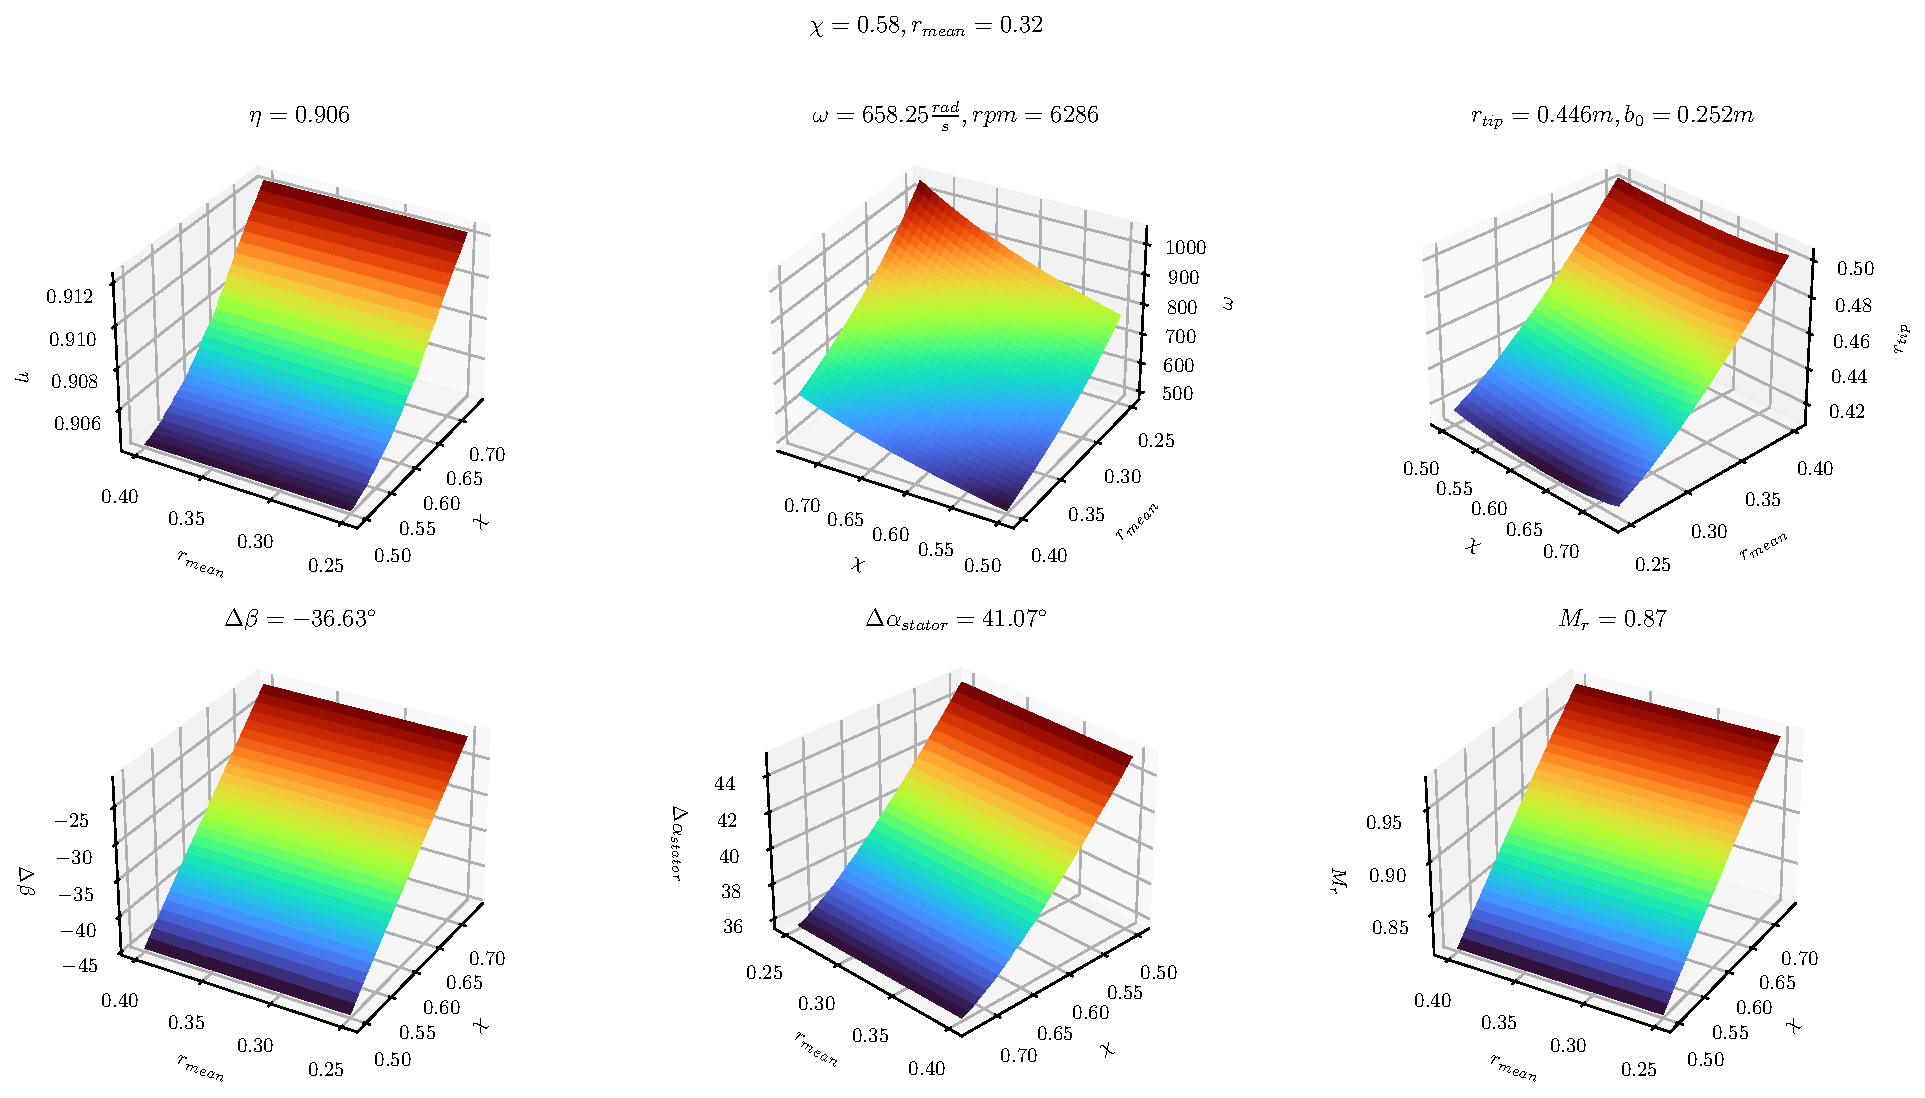
\includegraphics[width=\textwidth]{figures/rMeanChi.pdf}
		\end{figure}
	\end{frame}	

	\begin{frame}{Graph analysis: \textbf{rotor} $\alpha$, $\beta$ \& $V_{t}$}
		\begin{figure}
			\centering
			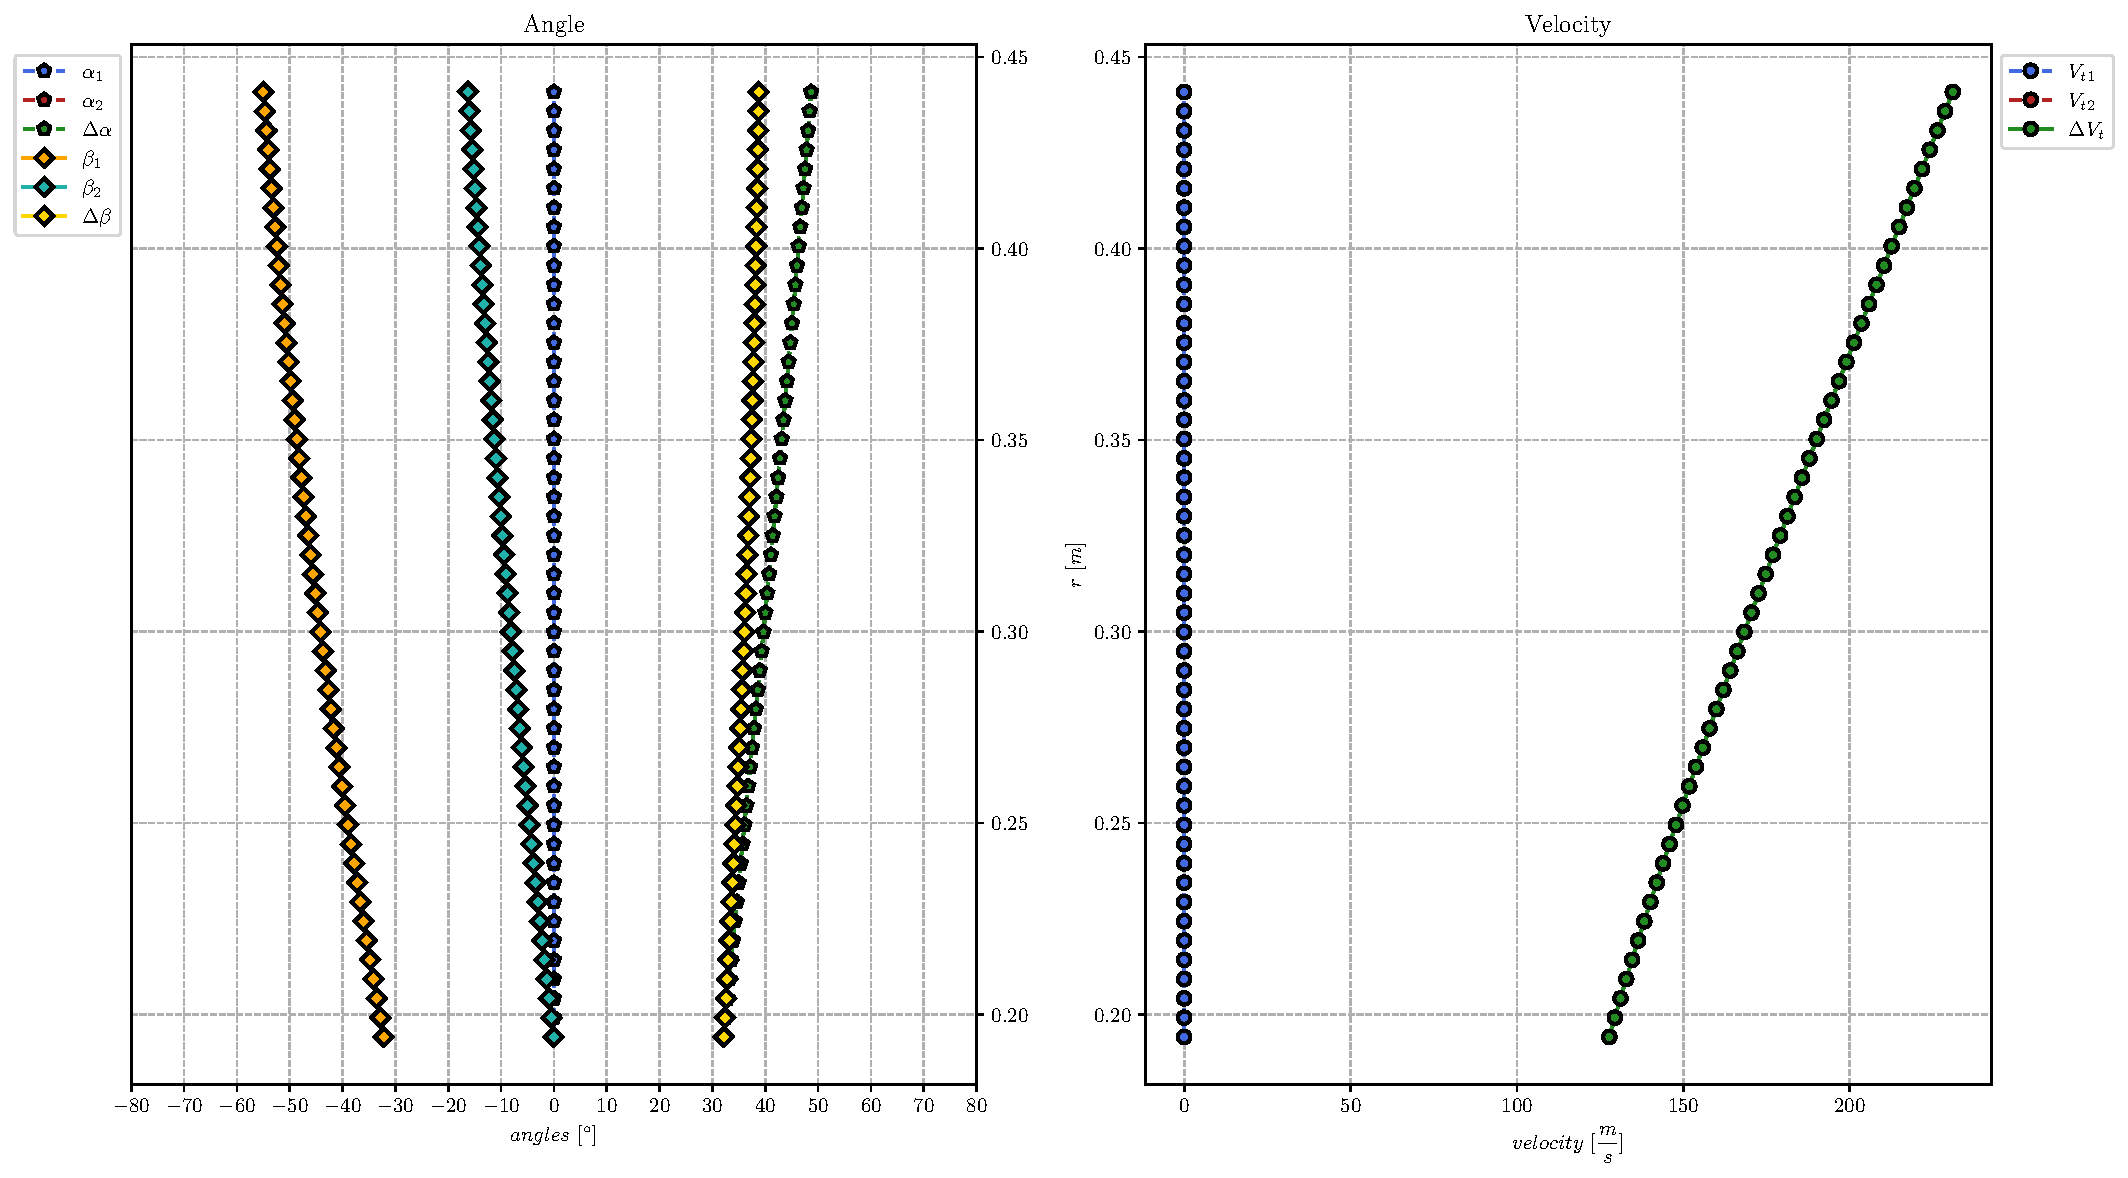
\includegraphics[width=\textwidth]{figures/betaAngles.pdf}
		\end{figure}
	\end{frame}
	
	\begin{frame}{Graph analysis: \textbf{stator} $\alpha$ \& $V_{t}$}
		\begin{figure}
			\centering
			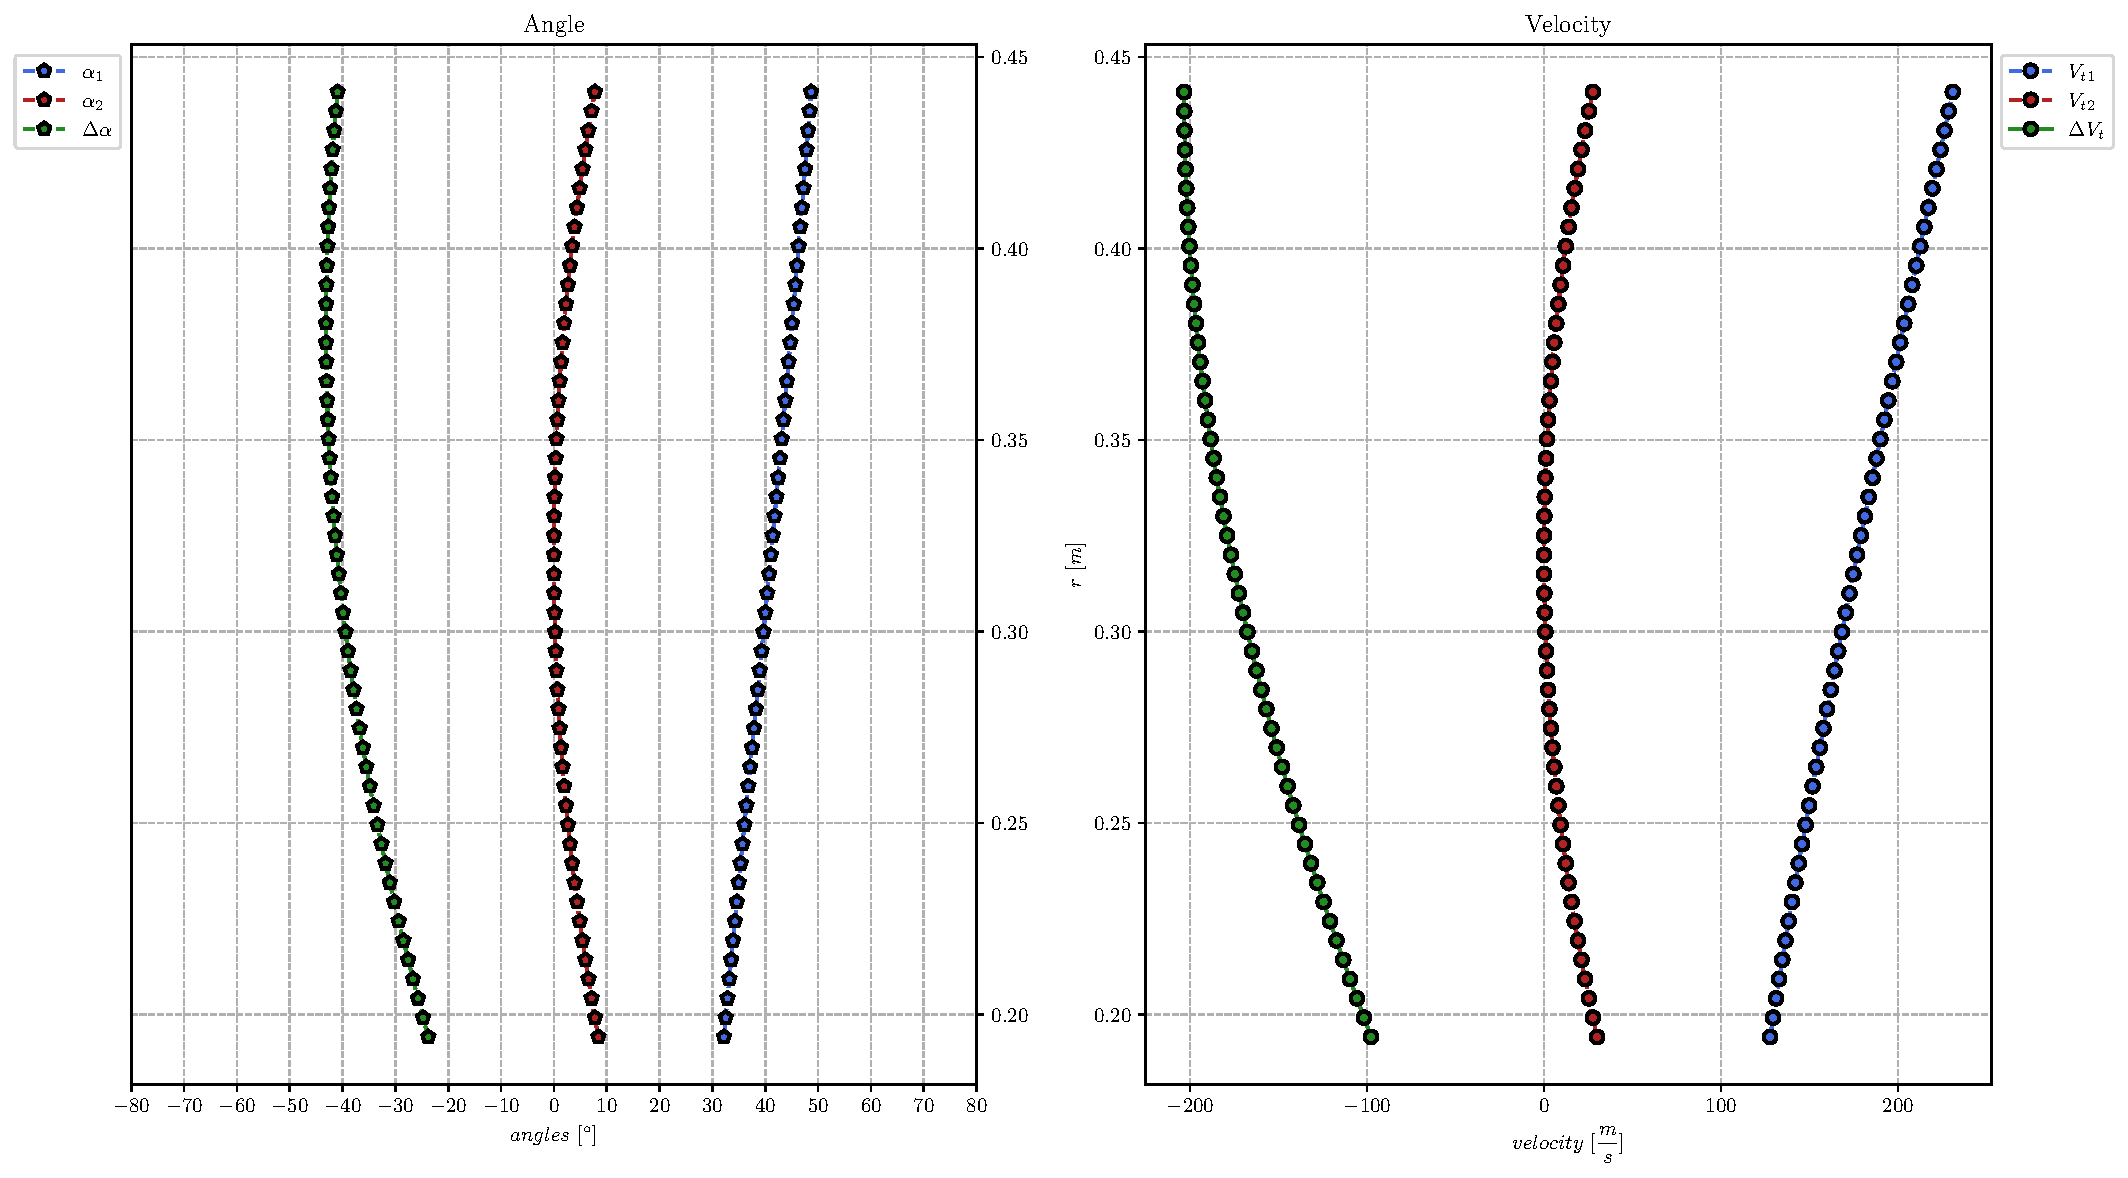
\includegraphics[width=\textwidth]{figures/alphaAngles.pdf}
		\end{figure}
	\end{frame}
	}

	\begin{frame}{$\lambda$ \& $\psi$}
		From the previous \textbf{graphs}:
		\begin{itemize}
            \item \footnote{\vspace{0.2cm}$\chi = \frac{h_1 - h_0}{h_{T1} - h_{T0}} = \frac{\frac{W_0^2}{2} - \frac{W_1^2}{2}}{U_{mean} (V_{t1} - V_{t0})} = \frac{\frac{W_{a0}^2}{2} + \frac{W_{t0}^2}{2}- \frac{W_{a1}^2}{2} - \frac{W_{t1}^2}{2}}{U_{mean} (V_{t1} - V_{t0})} = \frac{\frac{W_{t0}^2}{2} - \frac{W_{t1}^2}{2}}{U_{mean} (V_{t1} - V_{t0})}$}$\chi = 0.58$
			\item $r_{mean} = 0.32 m$
			\item $\frac{V_{t0}}{U_{mean}} = 0$
		\end{itemize}
		Taking into account the previous modeling \textbf{hypothesis}:
		\begin{align}
			\lambda & = \Bigg( 1 - \chi - \frac{V_{t0}}{U_{mean}} \Bigg) \cdot 4 \nonumber \\
			\psi    & = \frac{\lambda}{2} \nonumber
		\end{align}
	\end{frame}
	
	\begin{frame}{$\phi_{(\psi)}$}
		From \cite[Sec. 10.4]{axial2004} it is imposed that $\frac{W_2}{W_1} \geq 0.7$ with a \textit{safety} margin of $3 \%$. $\phi_{lim}$ line is related to the \textbf{surge safety margin}.  
		\begin{figure}
			\centering
			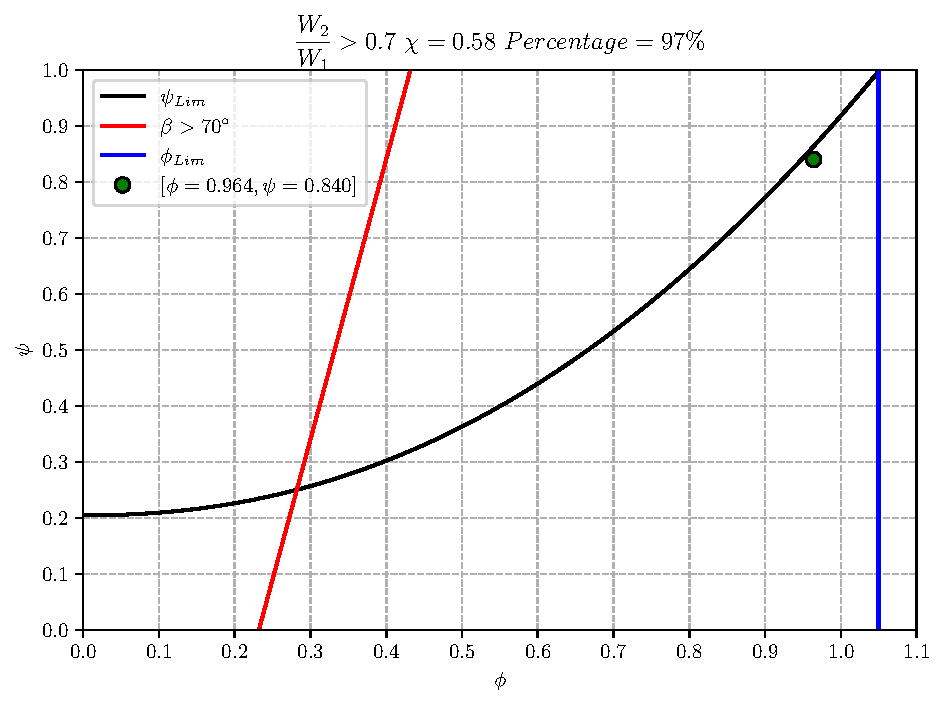
\includegraphics[width=0.7\textwidth]{figures/stagePerf.pdf}
		\end{figure}
	\end{frame}

	\begin{frame}{$\eta$ \& $L_{eu}$}
		$\eta$ is computed from an \textbf{Lieblein} efficiency chart\footnote{This chart has been interpolated from the course slides charts.} given $\phi$ and $\chi$. This parameter will be used for the computation of $L_{eu}$ given the $\beta_{TT}$ target.
		\begin{columns}
			\column{0.5\textwidth}
				\begin{figure}
					\centering 
					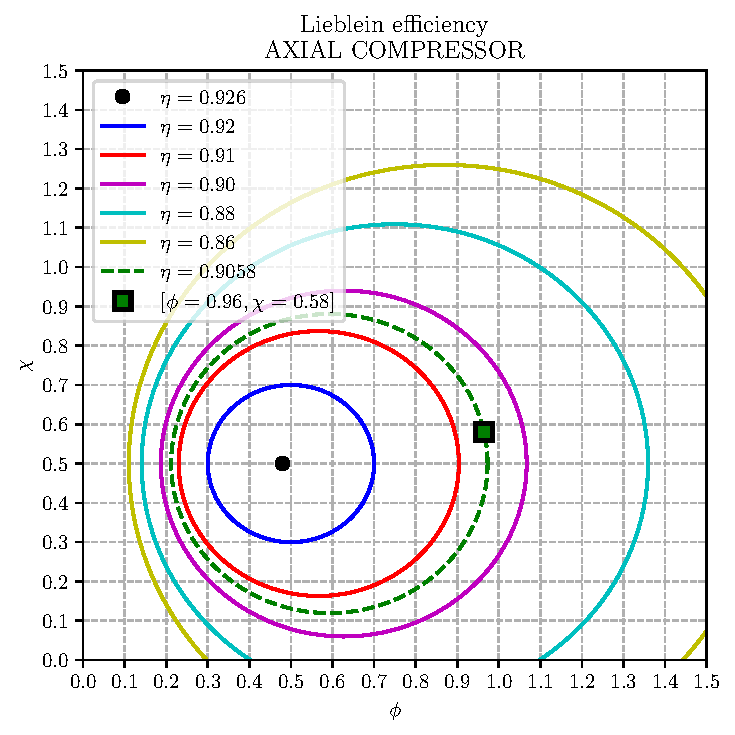
\includegraphics[width=1\textwidth]{figures/efficiency.pdf}
				\end{figure}
			\column{0.5\textwidth}
			\begin{align}
				L_{is} & = \frac{\gamma \ R}{\gamma - 1} \ T_{T0} \ (\beta_{TT}^{{\frac{\gamma - 1}{\gamma}}} - 1) \nonumber \\
				L_{eu} & = \frac{L_{is}}{\eta} \nonumber
			\end{align}
		\end{columns}
	\end{frame}

	\subsection{$V_{t_{mean}}$, $V_{a_{mean}}$, $U_{mean}$ \& velocity triangles}
\begin{frame}[fragile]{$V_{a_{mean}}$, $V_{t_{mean}}$ \& $U_{mean}$}
	\vspace{-0.8cm}
	\begin{align}
		U_{mean} & = \frac{L_{eu}}{\psi} \nonumber \\ 
		V_{a_{mean}} & = \phi \ U_{mean} \nonumber \\
		%L_{eu} & = U_1 \ V_{t1} - U_0 \ V_{t0} \nonumber \\ 
		L_{eu_{mean}} & = U_{1_{mean}} \ V_{t1_{mean}} - U_{0_{mean}} \ V_{t0_{mean}} \overset{U_1 = U_0}{=} U_{mean} \ \Delta V_{t_{mean}} \nonumber \\
		V_{t1_{mean}} & = \Delta V_{t_{mean}} + V_{t0_{mean}} \nonumber  
	\end{align}
	\vspace{-0.3cm}
	\begin{itemize}
		\item $\Delta V_{t_{mean}}$ computation allows us to get a \textit{first sketch} of the \textbf{velocity triangles}\footnote{\textbf{Mixed vortex} model and \textbf{second order} function based.} using $\phi$, $\psi$ and $L_{eu}$\footnote{$L_{eu} = U_1 \ V_{t1} - U_0 \ V_{t0}$} definitions. $V_a$ is assumed \textbf{constant} all through the stage.
		\item The first analysis results are stored in \verb|compressor_0.58_0.32_45_35.txt|
	\end{itemize}
\end{frame}

%\begin{frame}{Nomenclature}
%    \scriptsize{
%        \begin{itemize}
%            \item $\mathtt{0, 1, 2}$: rotor inlet, rotor outlet/stator inlet, stator outlet
%            \item $P_{T0}$: inlet total pressure 
%            \item $T_{T0}$: inlet total temperature
%            \item $r_{max}$: max rotor/stator tip radius
%            \item $\beta_{TT}$: pressure ratio expressed in total pressure 
%            \item $\dot{m}$: mass flux 
%            \item $\eta$: efficiency
%            \item $\psi$: stage work coefficient
%            \item $\phi$: stage flow coefficient 
%            \item $\chi$: reaction degree 
%            \item $\omega$: rotation speed 
%            \item $V_{*}$: absolute speed at $\mathtt{*}$ station
%            \item $V_{a*}$: axial absolute speed at $\mathtt{*}$ station
%            \item $V_{t*}$: tangential absolute speed at $\mathtt{*}$ station 
%            \item $W_{*}$: relative speed at $\mathtt{*}$ station
%            \item $W_{a*}$: axial relative speed at $\mathtt{*}$ station
%            \item $W_{t*}$: tangential relative speed at $\mathtt{*}$ station 
%            \item $L_{is}$: isentropic work 
%            \item $L_{eu}$: real work 
%            \item $U_{mean}$: rotational speed at meanline 
%            \item $\gamma$: specific heat ratio 
%            \item $R$: gas constant
%        \end{itemize}
%    }
%\end{frame}

    
   	\section{Models}
        \subsection{Losses Modeling}
\subsubsection{Profile Losses}
	\begin{frame}{Profile Losses}
		The profile losses used are related to the \textbf{Leiblein modeling} approach, \cite[Ch. 6]{axial2004}.
				
	\end{frame}
\subsubsection{Compressibility Losses}
\subsubsection{Shock Losses}
\subsubsection{Tip Leackage Losses}
\subsection{Radial Equilibrium}
\subsubsection{General Formulation}
\subsubsection{Vortex Model}
\subsubsection{$\mathtt{NISRE}$ Equilibrium Results}
\subsection{$\mathtt{turboLIB}$}
\subsubsection{Section Analysis \& Optimization}
\subsubsection{$\mathtt{.stl}$ \& $\mathtt{.scad}$ Generation}


	
	\section{\texttt{turboLIB} \& Results}
		\subsection{$\mathtt{turboLIB}$}
	\begin{frame}[fragile]{$\mathtt{turboLIB}$}
		The preliminary compressor design model program \href{https://github.com/antoniopucciarelli/turboLIB}{\color{blue}{$\mathtt{turboLIB}$}} can be downloaded from GitHub.
		\begin{block}{Main objects and modules}
			\begin{itemize}
				\item \verb|turboClass.turboBlade.blade|: blade object
				\item \verb|turboCoeff|: engineering coefficients module
					\begin{itemize}
						\item \verb|losses|: losses modeling 
						\item \verb|similarity|: adimensional analysis
						\item \verb|lieblein|: blade modeling
					\end{itemize}
				\item \verb|geometry.bladeGeometry.geometryData|: airfoil object
			\end{itemize}
		\end{block}
	\end{frame}

\subsubsection{Blade number}
	{\nologo
	\begin{frame}{Blade number}
		In order to define a proper number of blades for the rotor and the stator, \textbf{Howell}'s relations have been used for the estimation of the \textbf{losses}. These relations, \cite[Ch. 6]{axial2004}, are:
		\begin{itemize}
			\item $\bar{\omega}_{profile + secondary}$, this is a relation that takes into account \textbf{profile} and \textbf{3D} losses
			\item $\bar{\omega}_{endWall}$, this is previous expalined \textbf{end wall} loss
		\end{itemize}
		
		\begin{columns}
			\column{0.5\textwidth}
			\begin{figure}
				\centering
				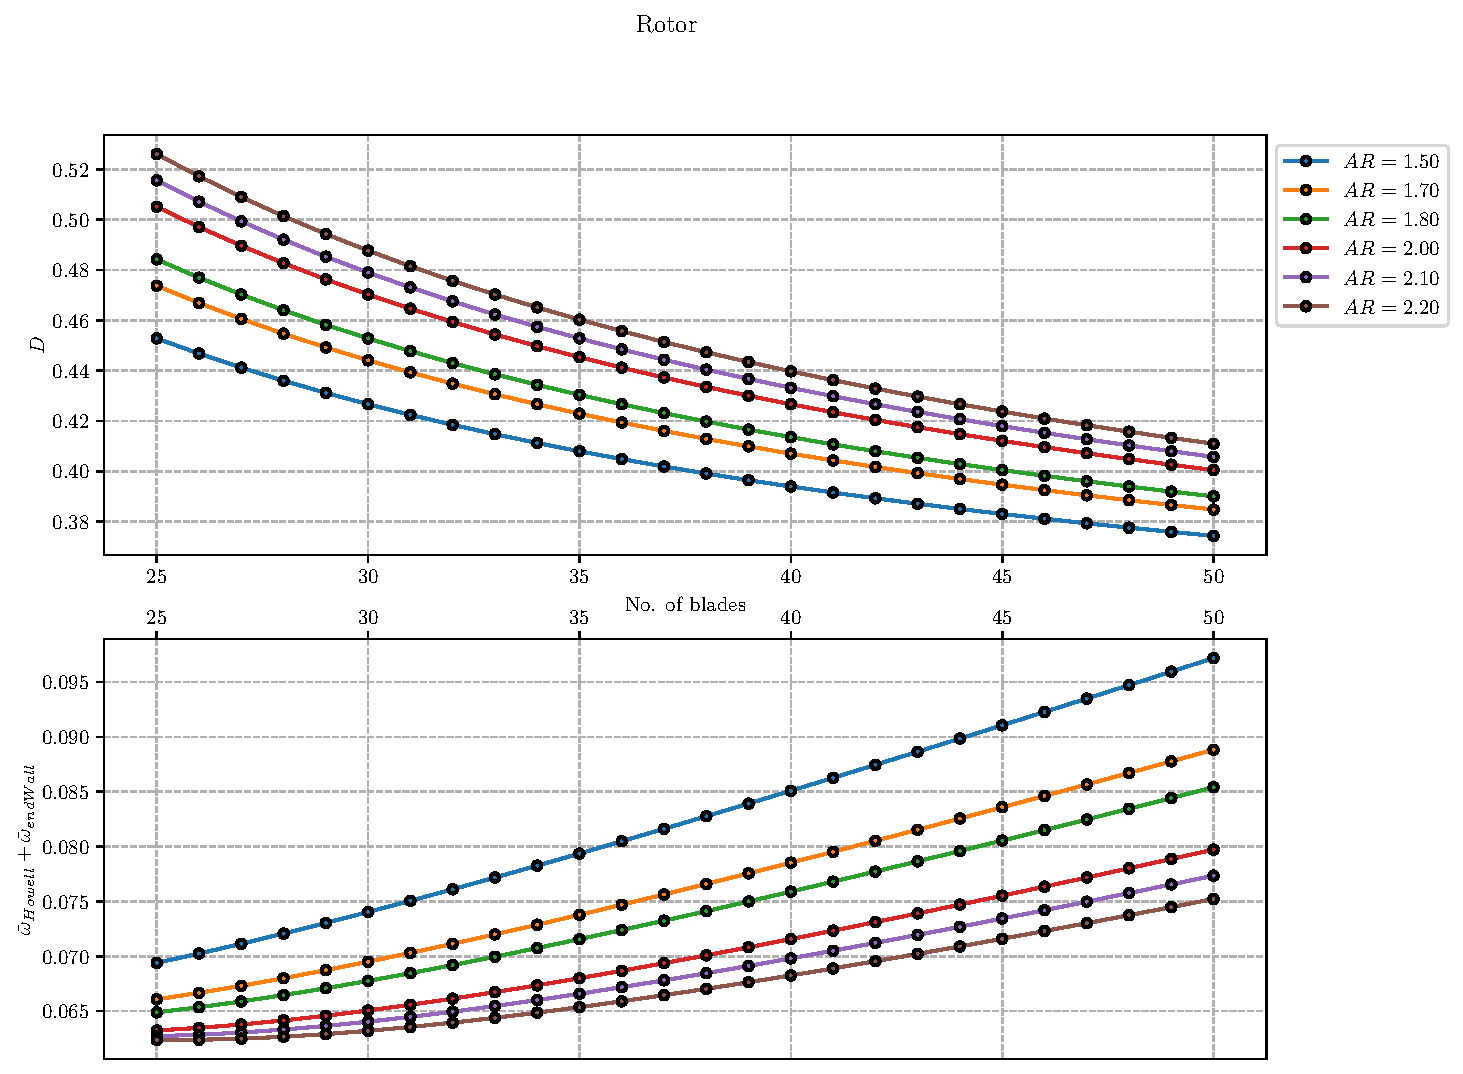
\includegraphics[width=1\textwidth]{figures/rotorBlades.pdf}
			\end{figure}
			\column{0.5\textwidth}
			\begin{figure}
				\centering
				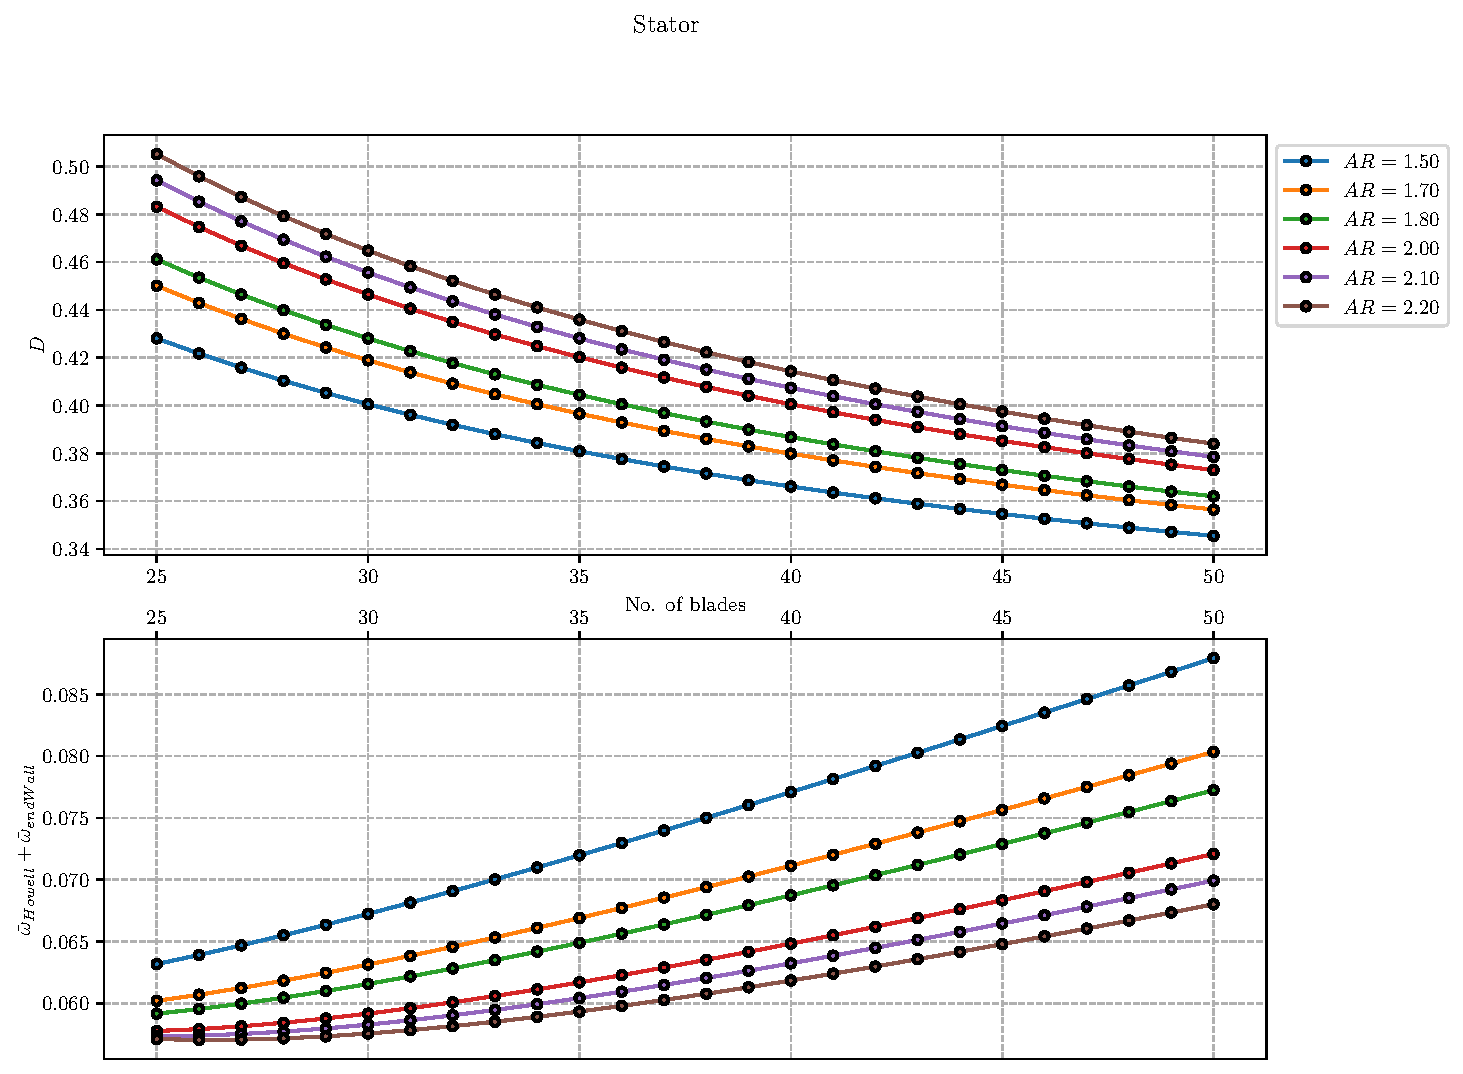
\includegraphics[width=1\textwidth]{figures/statorBlades.pdf}
			\end{figure}
		\end{columns}
	\end{frame}
	}
\subsubsection{$\mathtt{NISRE}$ results}
	\begin{frame}[fragile]{$\mathtt{NISRE}$ setup}
		The \verb|NISRE| is solved through a \textbf{double nested} loop:
		\begin{itemize}
			\item \textbf{continuity loop}
			\item \textbf{entropy loop}
		\end{itemize}
		Inside the \textbf{continuity loop} the \verb|scipy.integrate.odeint| function is used for the solution of the $V_{a2}^2$ \textbf{ODE}.
		\newline
		\newline
		Inside the \textbf{entropy loop} the \verb|scipy.optimize.minimize| function is used for the computation of the blade \textbf{shape}.
	\end{frame}

\subsubsection{$\mathtt{.stl}$ \& $\mathtt{.scad}$ generation}
	\begin{frame}[fragile]{$\mathtt{.stl}$ \& $\mathtt{.scad}$ generation}
		At the end of the \verb|NISRE|, all the main blade quantities are avaliable for the \textbf{generation} of the \textbf{3D geometry}. This geometry can be converted into a \verb|.stl| file that can be used in \verb|OpenFOAM| for the flow properties study. In addition a \verb|.scad| file is made for understanding position and checking possible contacts between rotor and stator blades.	
		\newline
		\newline 
		\cite{baskharone2006principles} suggested that a good distance between rotor and stator blades is half of the rotor chord\footnote{In the radial equilibrium study losses between rotor \newline and stator blades are \textbf{neglected}.}.
	\end{frame}

\subsection{Results}
	\subsubsection{$\mathtt{NISRE}$ and main quantities}
	\begin{frame}{\textbf{Rotor} equilibrium results: $\mathtt{NISRE}$}
		\begin{figure}
			\centering
			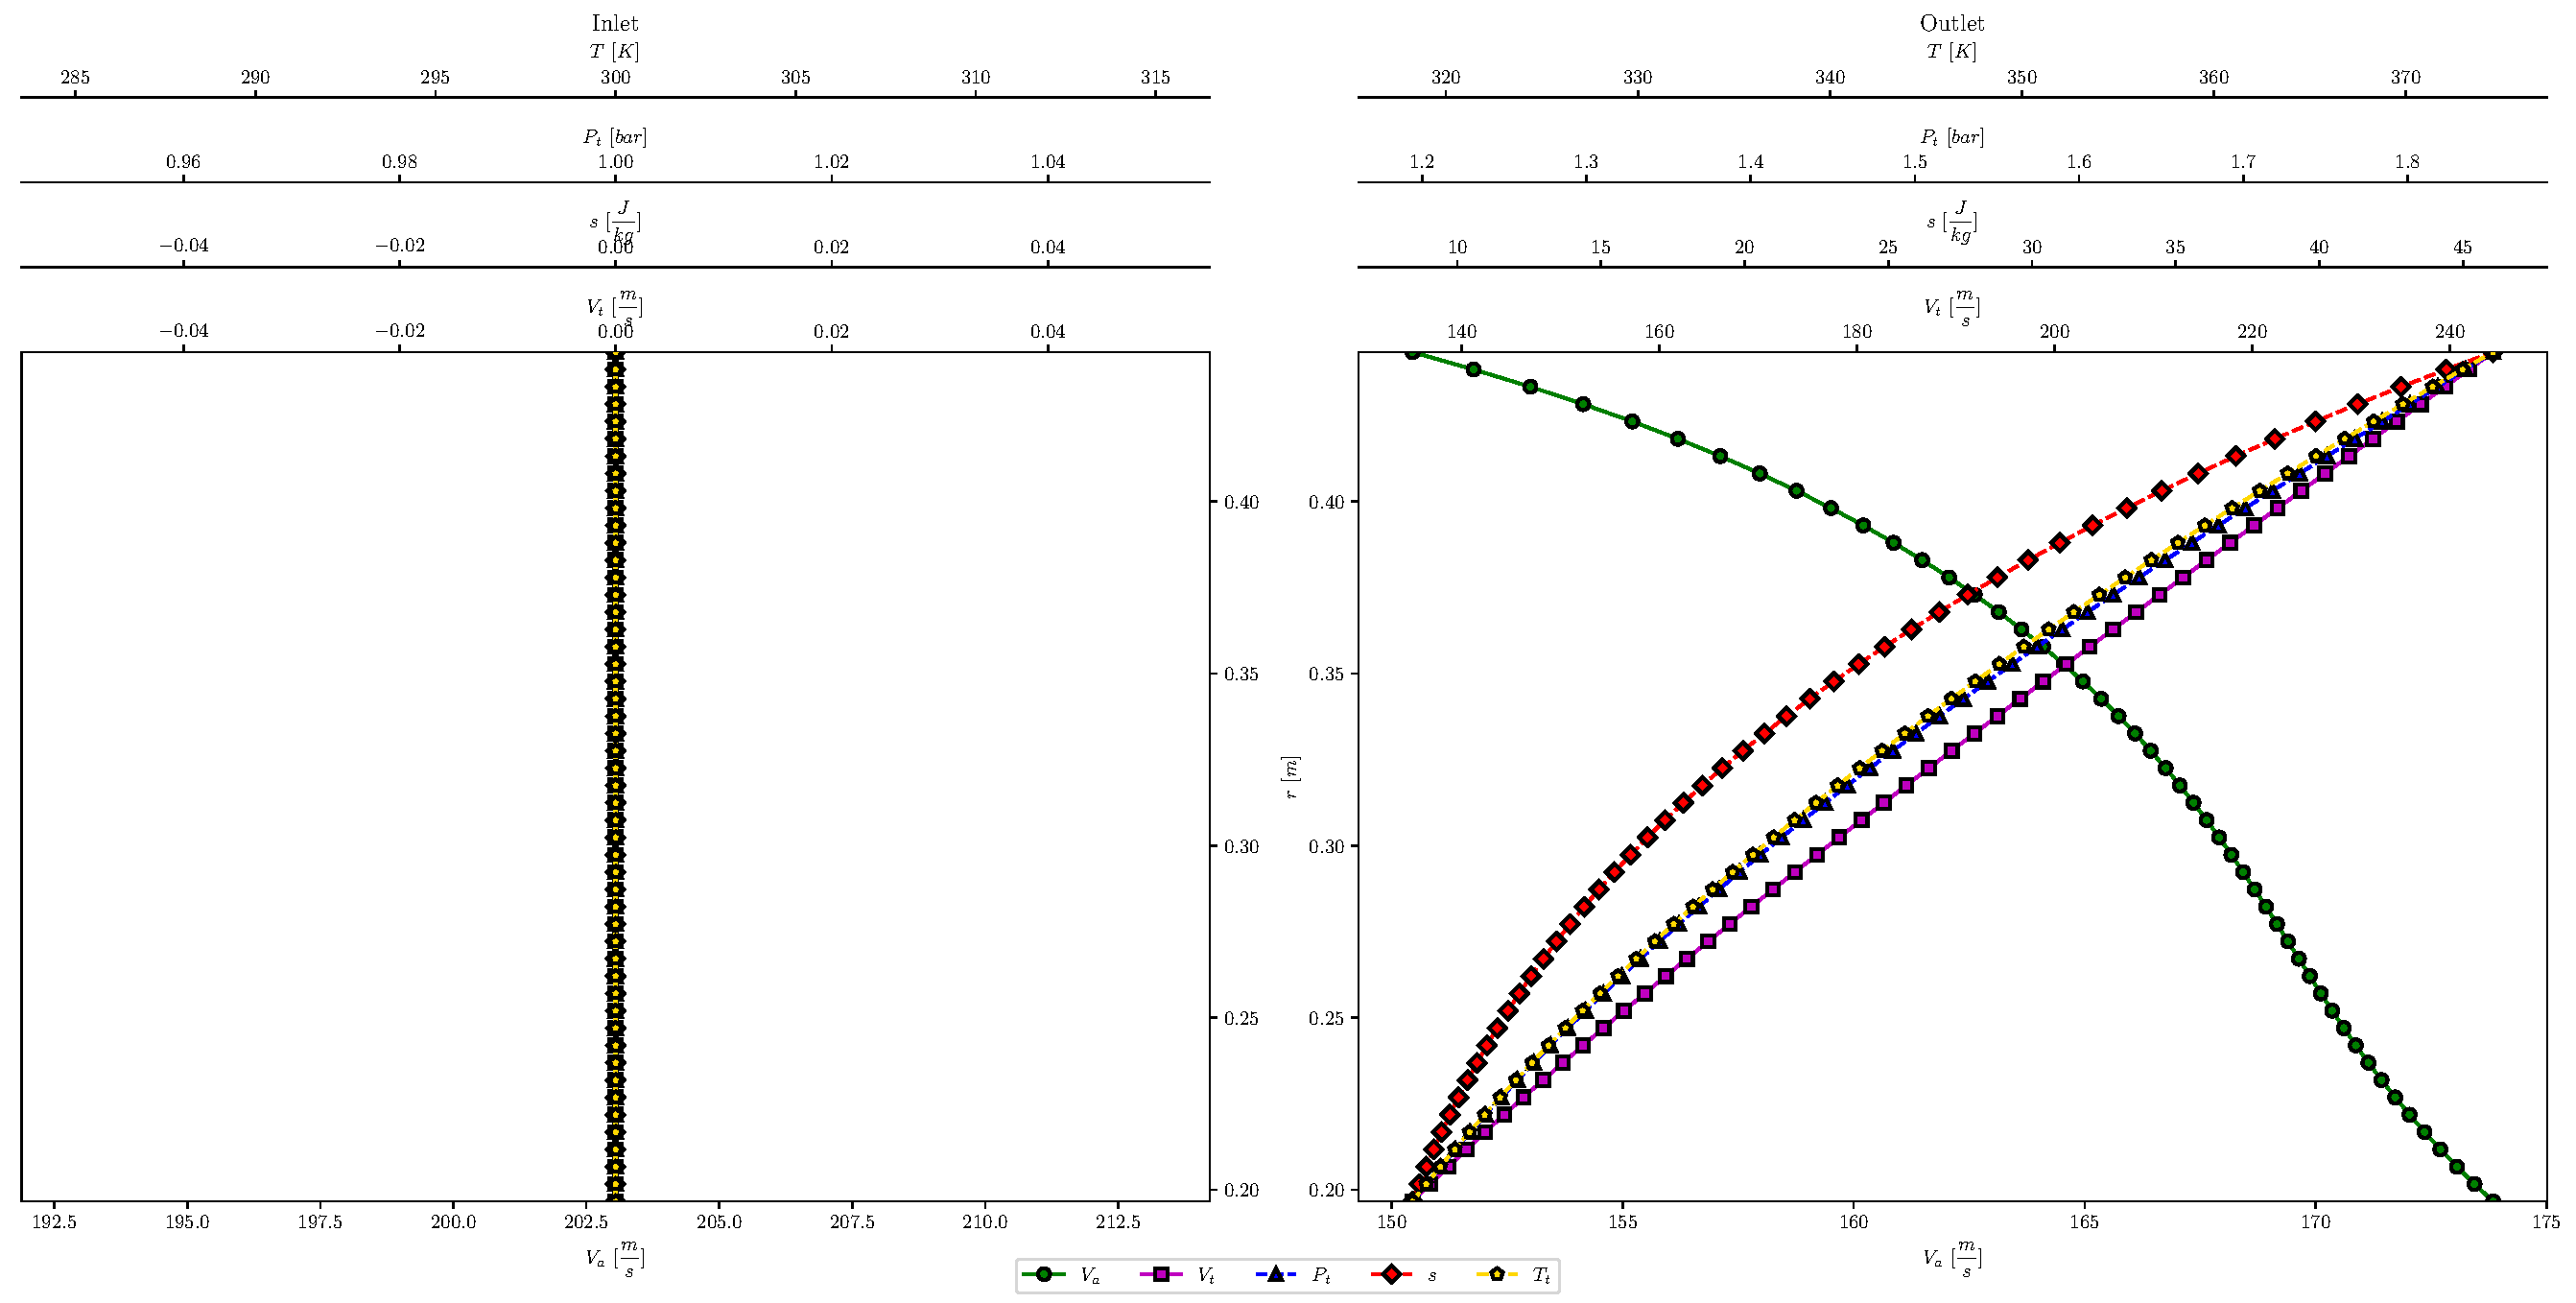
\includegraphics[width=1\textwidth]{figures/rotorEntropyFlow.pdf}
		\end{figure}
	\end{frame}
	
	\begin{frame}{\textbf{Rotor} equilibrium results: main quantities}
		\begin{figure}
			\centering
			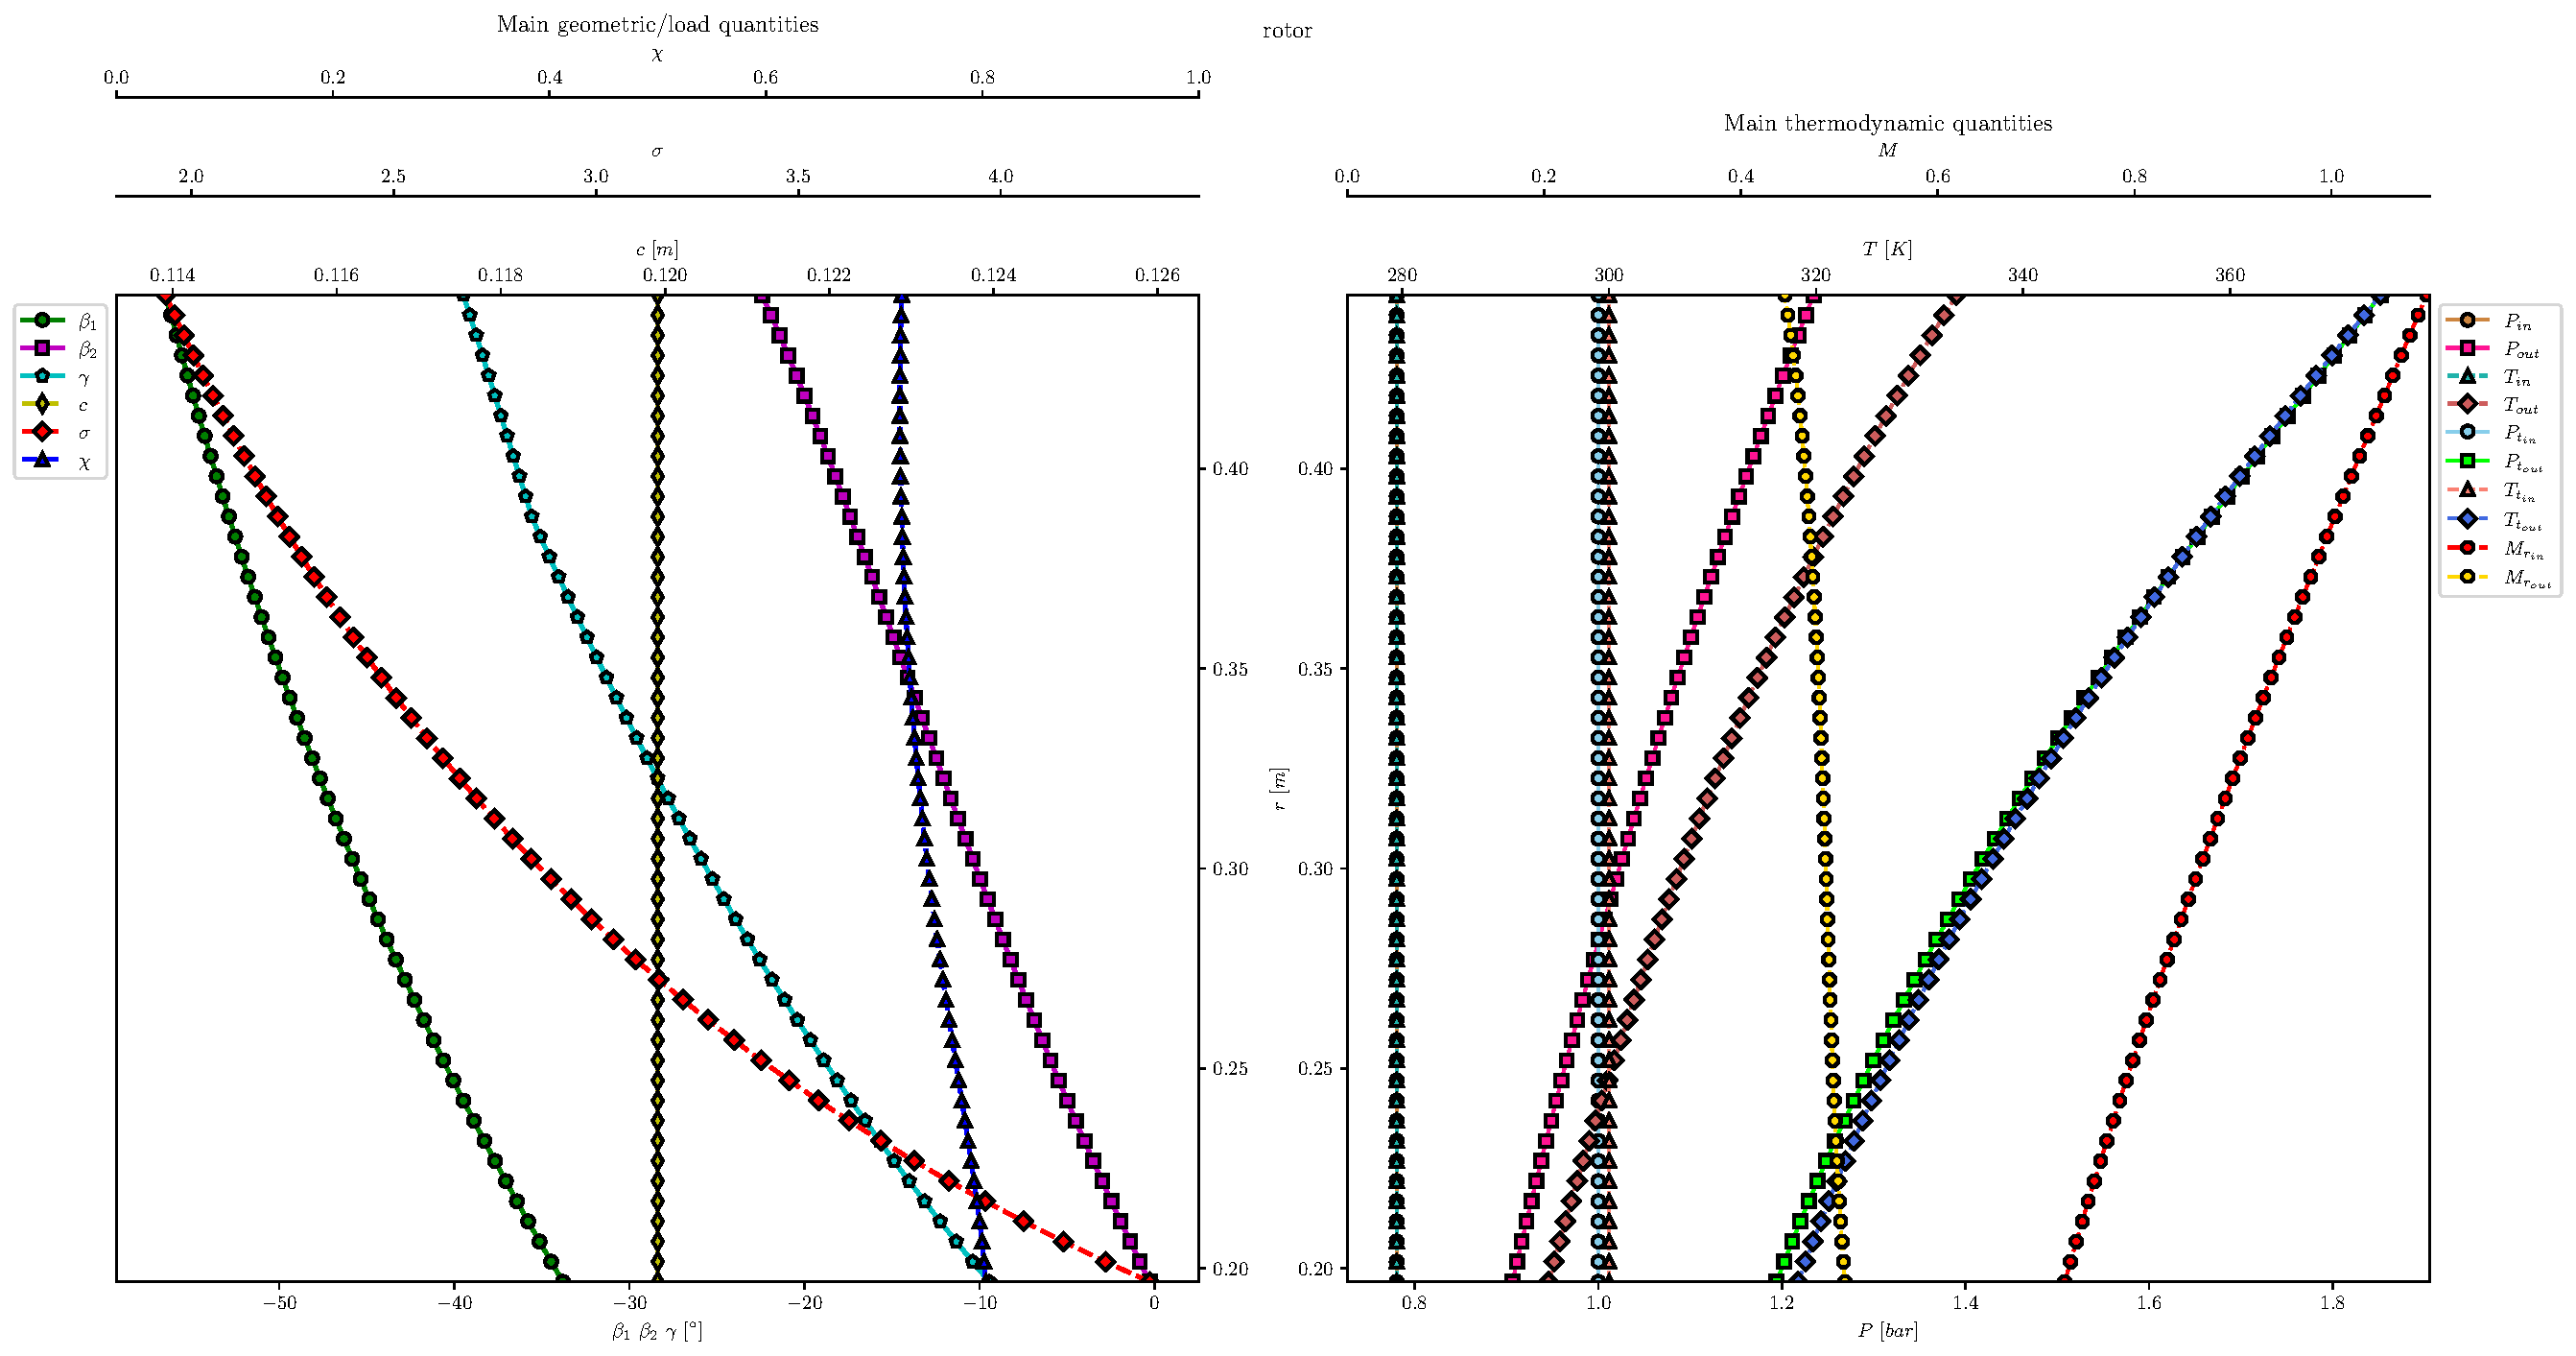
\includegraphics[width=1\textwidth]{figures/rotorBetaThermo.pdf}
		\end{figure}
	\end{frame}
	
	\begin{frame}{\textbf{Stator} equilibrium results: $\mathtt{NISRE}$}
		\begin{figure}
			\centering
			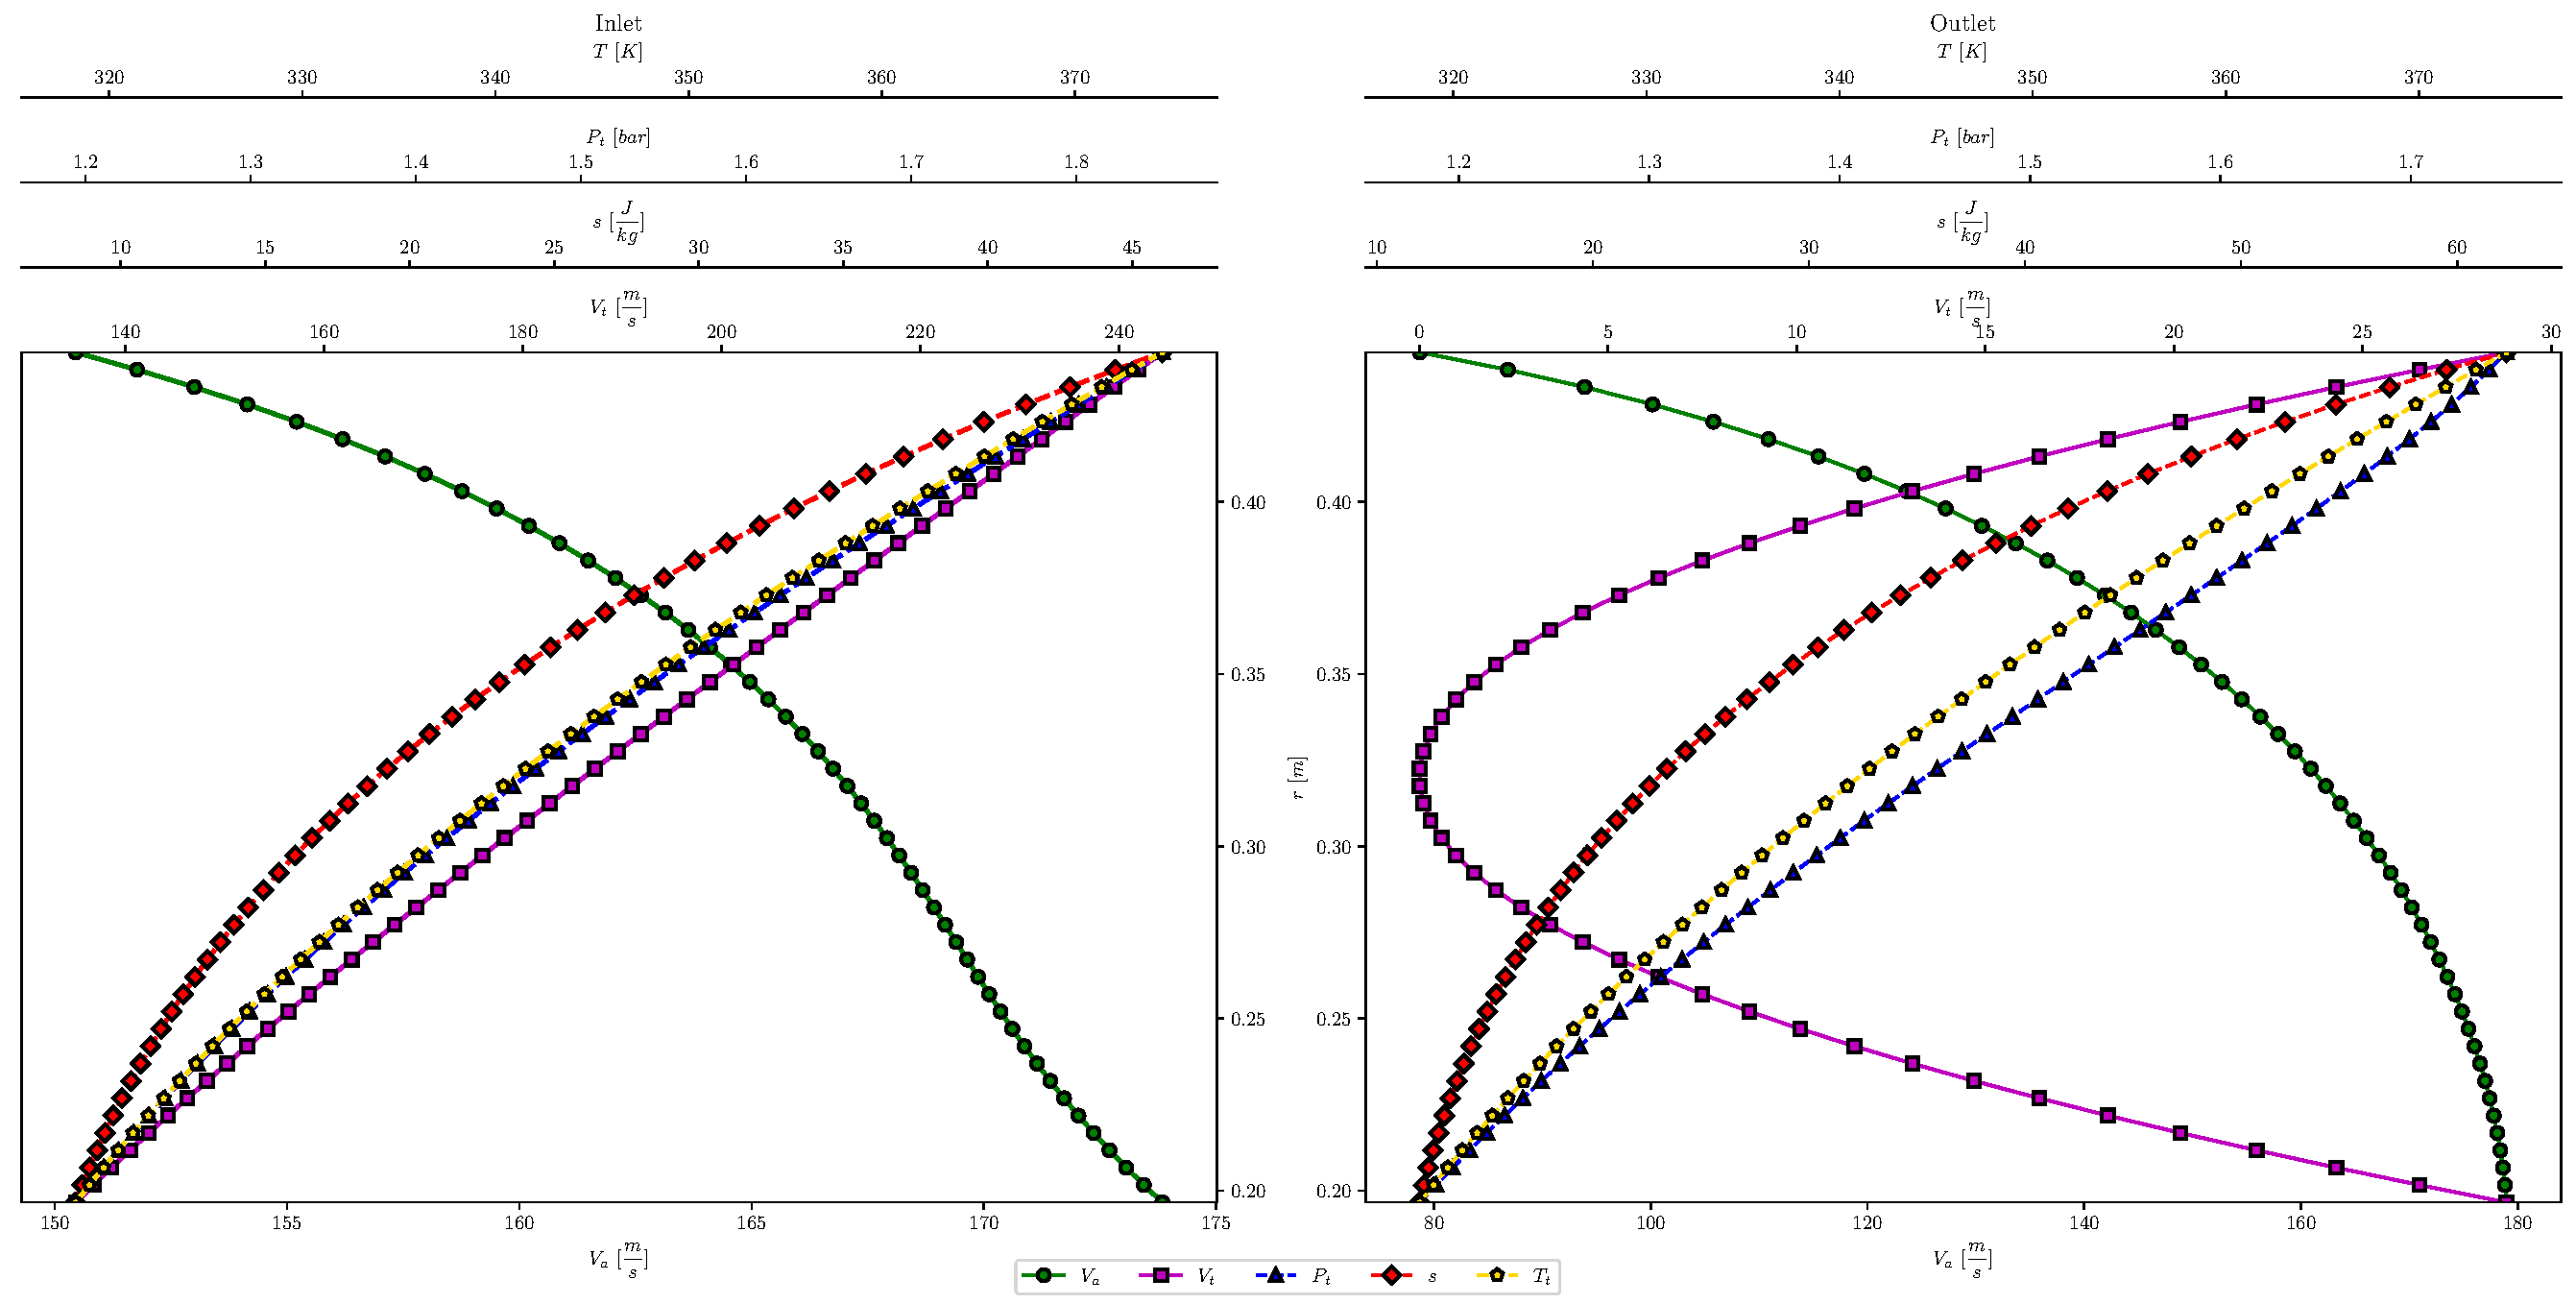
\includegraphics[width=1\textwidth]{figures/statorEntropyFlow.pdf}
		\end{figure}
	\end{frame}
	
	\begin{frame}{\textbf{Stator} equilibrium results: main quantities}
		\begin{figure}
			\centering
			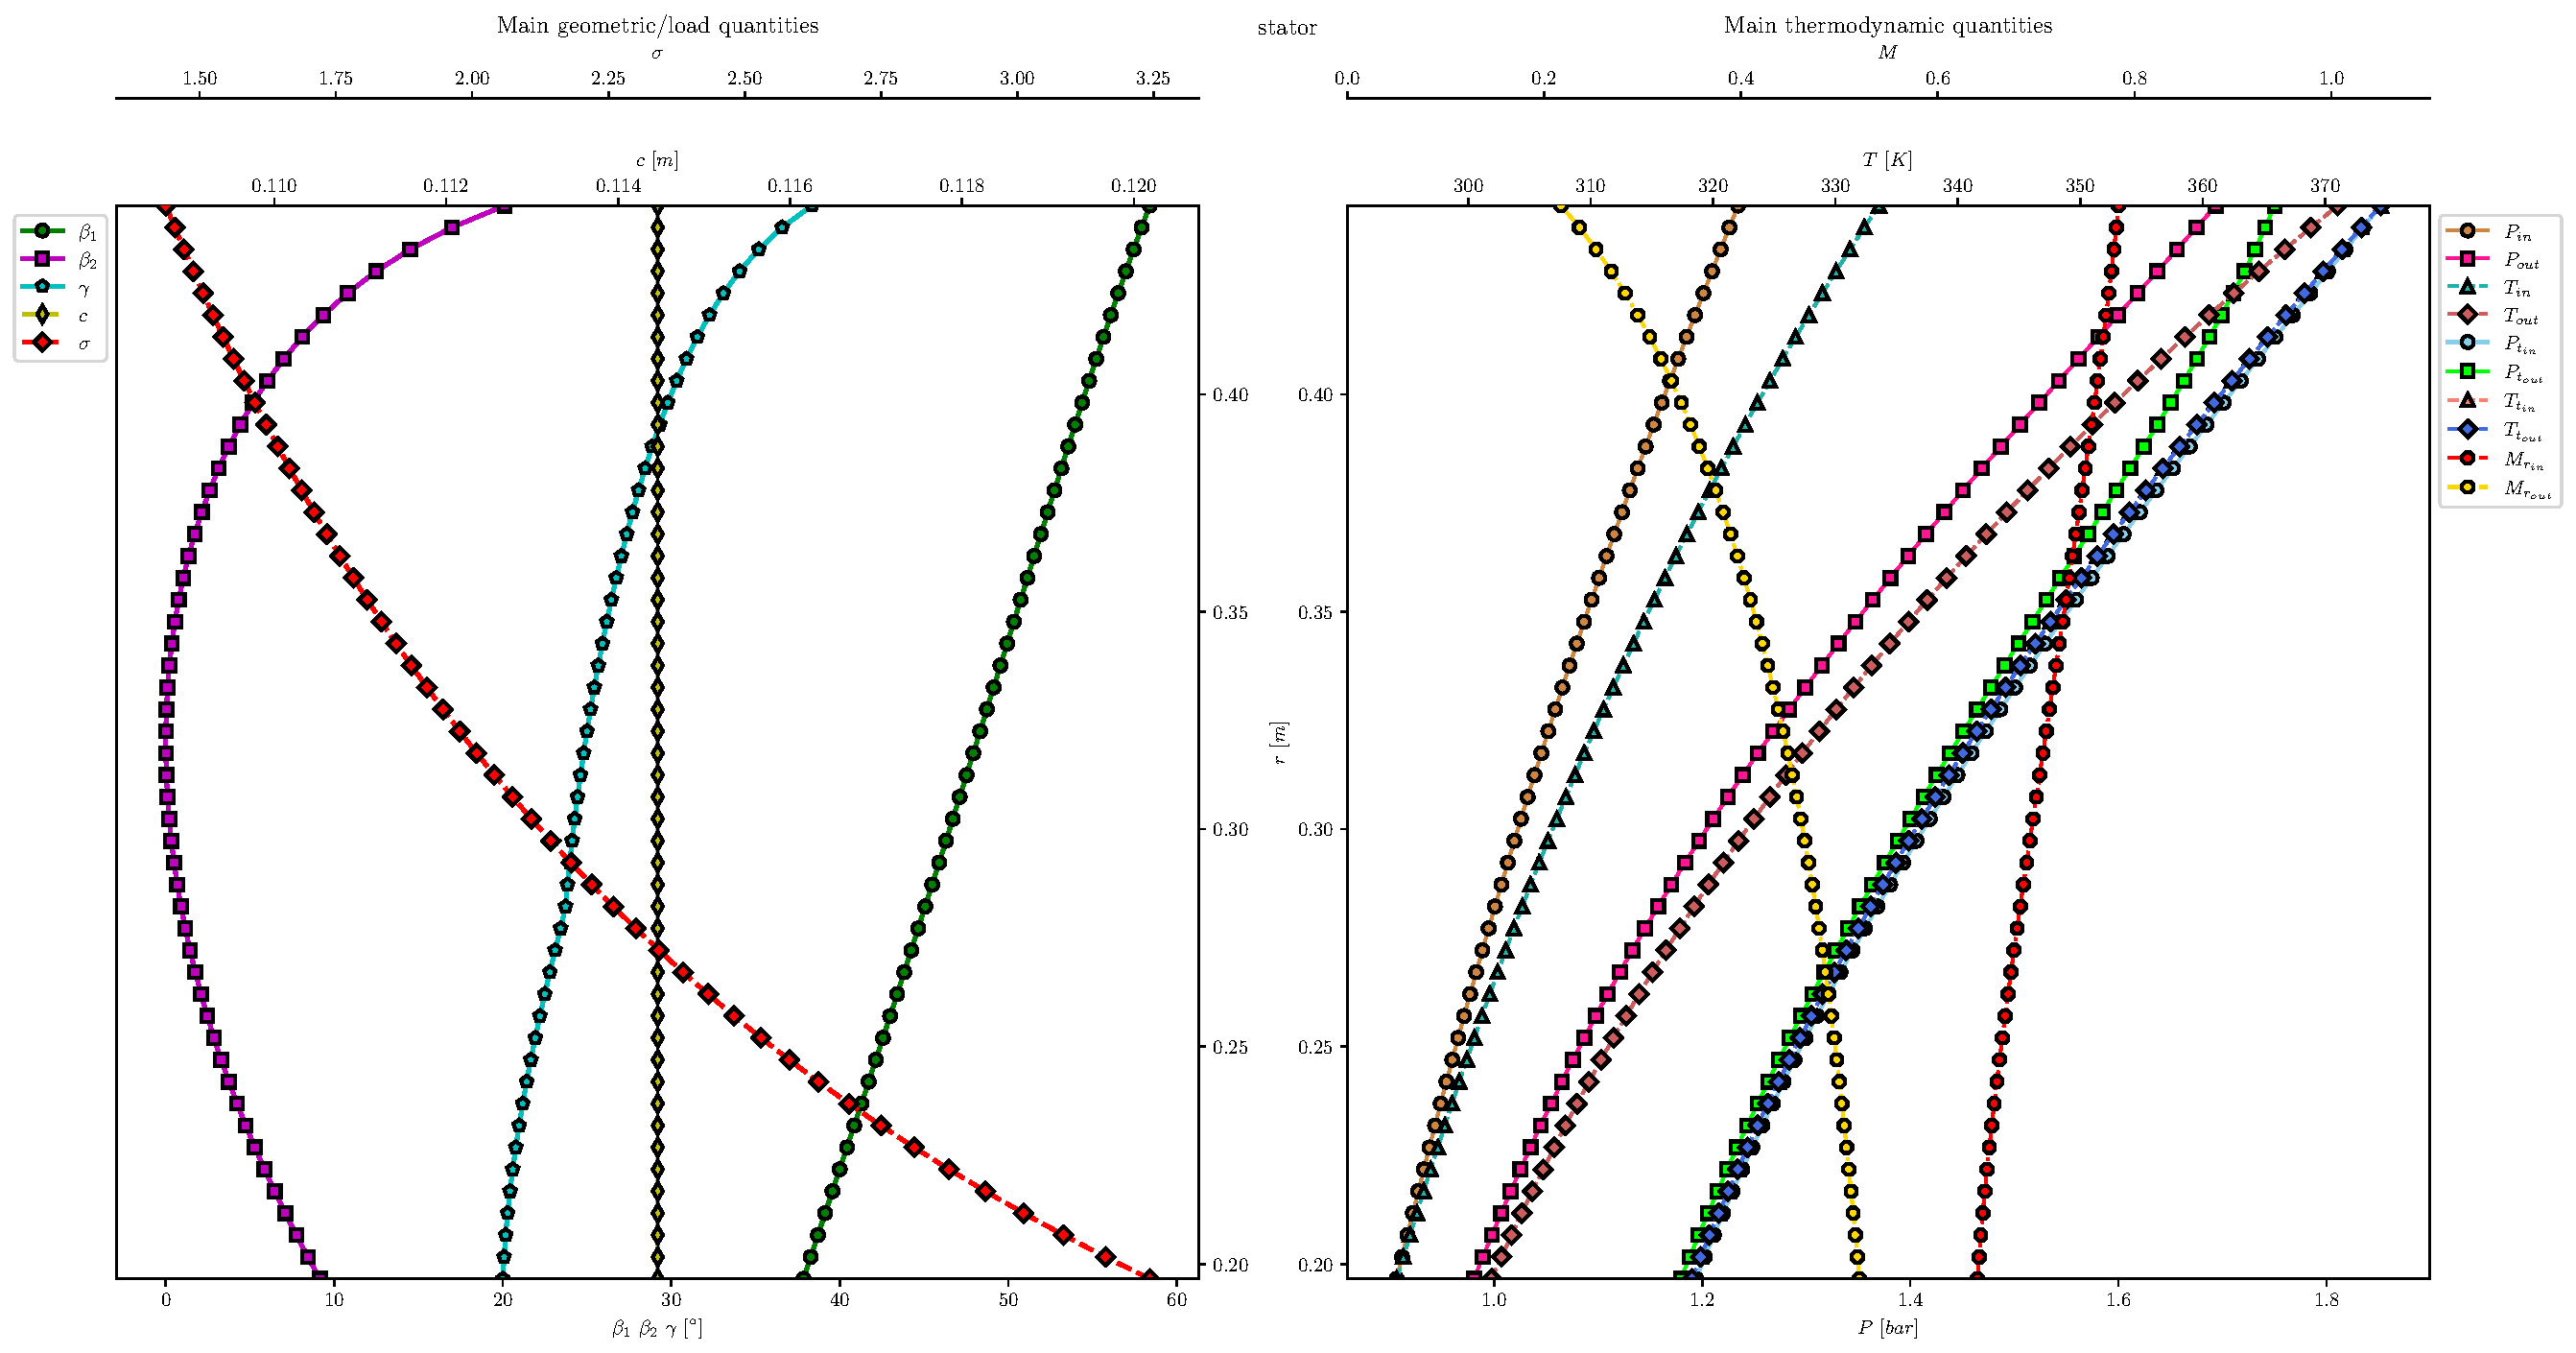
\includegraphics[width=1\textwidth]{figures/statorBetaThermo.pdf}
		\end{figure}
	\end{frame}
	
	{\nologo
	\begin{frame}{Velocity triangles}
		\begin{columns}
			\column{0.5\textwidth}
				\begin{itemize}	
					\item Inlet: \textbf{free vortex} model
					\item Outlet: \textbf{mixed vortex} model
				\end{itemize}
				\begin{figure}
					\centering
					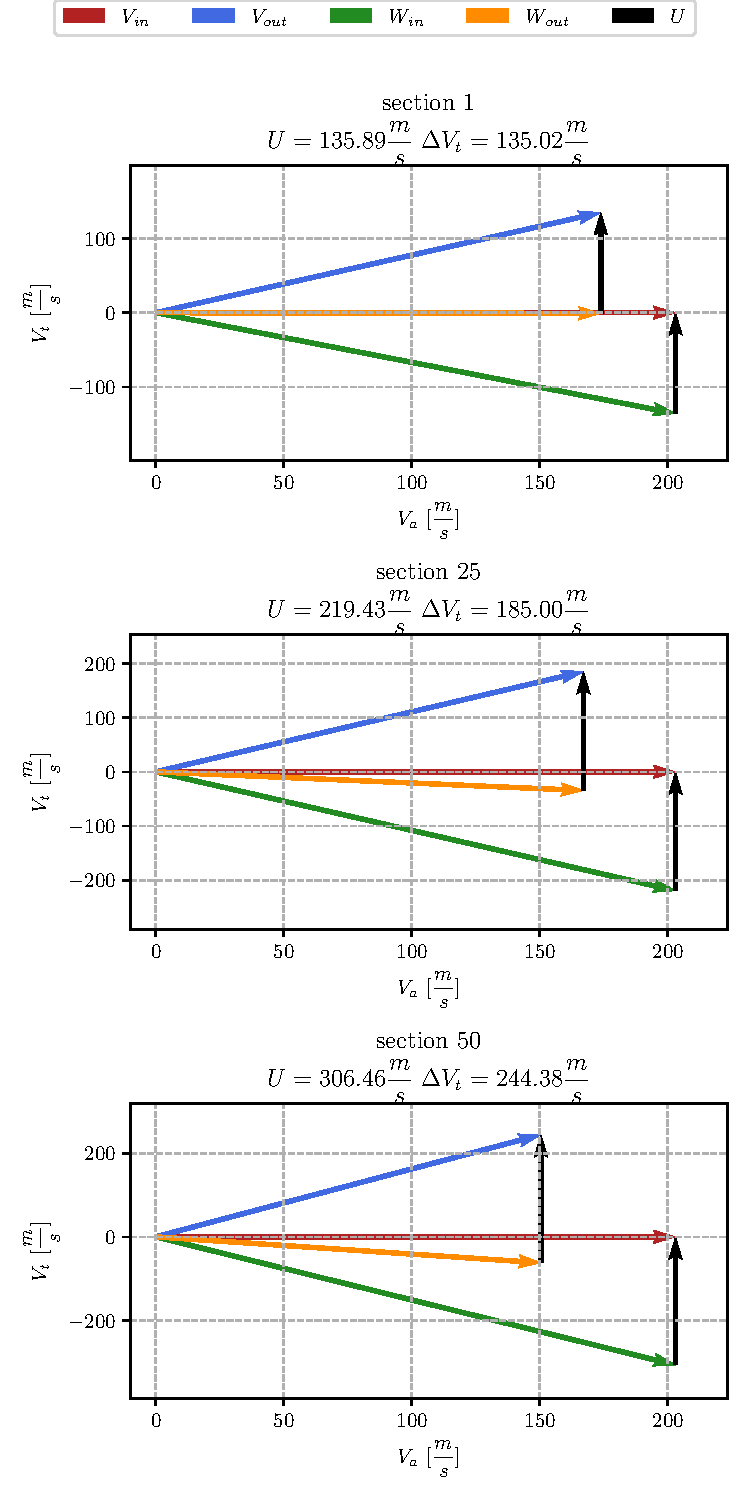
\includegraphics[width=0.5\textwidth]{figures/rotorVelocityTriangle.pdf}
				\end{figure}
			\column{0.5\textwidth}
				\begin{itemize}	
					\item Inlet: \textbf{mixed vortex} model
					\item Outlet: \textbf{second order} function 
				\end{itemize}
				\begin{figure}
					\centering
					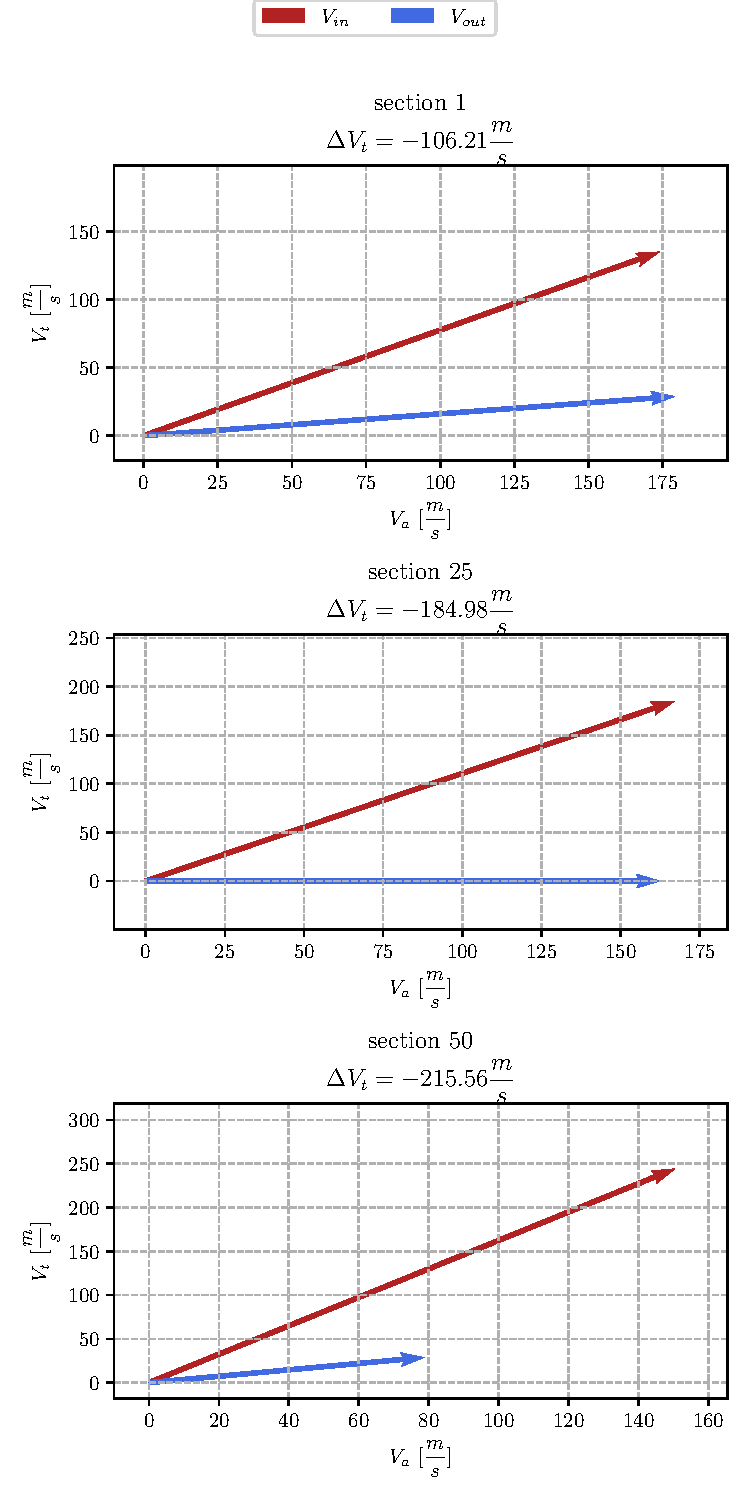
\includegraphics[width=0.5\textwidth]{figures/statorVelocityTriangle.pdf}
				\end{figure}
		\end{columns}
	\end{frame}
	}
	
	\begin{frame}{\textbf{Rotor} \& \textbf{stator} blades}
		\begin{columns}
			\column{0.5\textwidth}
				\begin{figure}
					\hspace{-2cm}
					\includegraphics[width=1.5\textwidth]{figures/rotor.png}
					\caption{Rotor blade.}
				\end{figure}
			\column{0.5\textwidth}
				\begin{figure}
					\hspace{-2cm}
					\includegraphics[width=1.5\textwidth]{figures/stator.png}
					\caption{Stator blade.}
				\end{figure}
		\end{columns}
	\end{frame}
	
	\begin{frame}{\textbf{Stage} plot}
		\begin{figure}
			\centering
			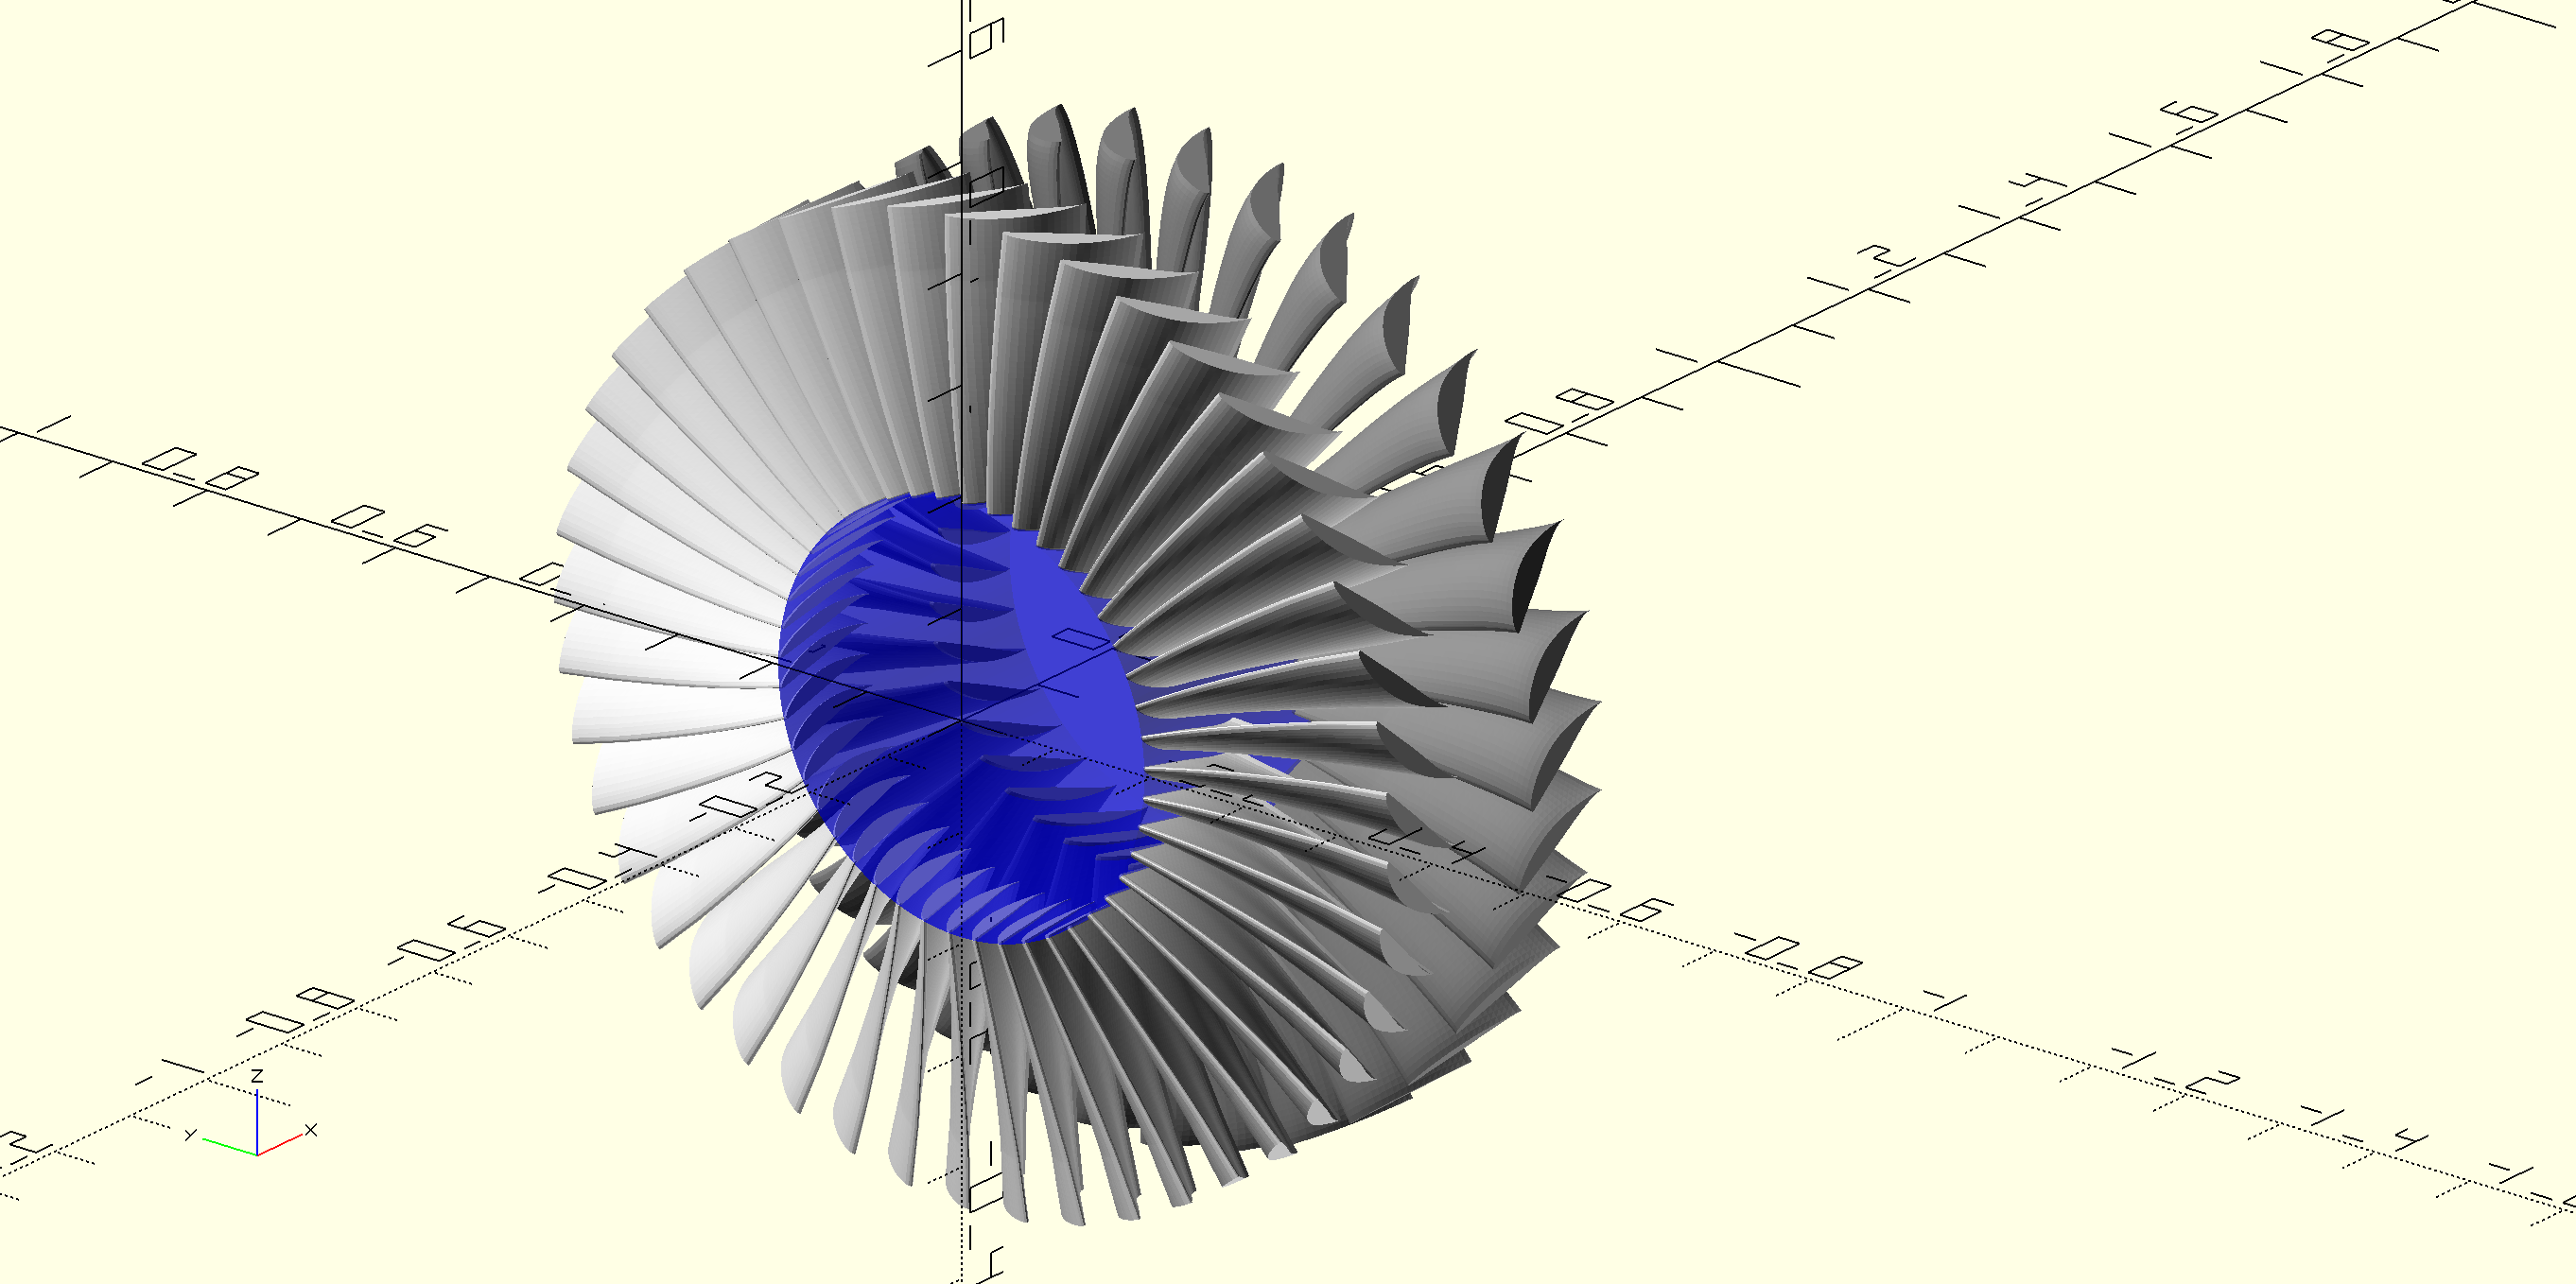
\includegraphics[width=1\textwidth]{figures/compressor.png}
		\end{figure}
	\end{frame}

\subsubsection{Efficiency}
	\begin{frame}[fragile]{Efficiency}
		The \textbf{rotor} efficiency is computed with:
		\begin{equation}
			\eta_{is_{rotor}} = \frac{W_1^2 - W_{2_{is}}^2}{W_1^2 - W_{2}} \nonumber 
		\end{equation}
		The \textbf{stator} efficiency is computed with:
		\begin{equation}
			\eta_{is_{stator}} = \frac{\Delta h_{is}}{\Delta h_{real}}
			\nonumber 
		\end{equation}
		The modeling results are stored into \verb|compressor_0.55_0.325_28_28.txt|.
	\end{frame}


	%\section{CFD}
	%\input{verification}
	    
	\begin{frame}[allowframebreaks]
		\printbibliography
	\end{frame}

	\begin{frame}
		\begin{center}
			{\Huge \emph {\textrm{Thank  ~you!}}}
		\end{center}
		
		\vspace{2cm}
		
		\Large{\textbf{Antonio Pucciarelli} \hfill 974675} \\ 
        
	\end{frame}
\end{document}
